%!TEX root = ../template.tex
%%%%%%%%%%%%%%%%%%%%%%%%%%%%%%%%%%%%%%%%%%%%%%%%%%%%%%%%%%%%%%%%%%%%
%% chapter4.tex
%% NOVA thesis document file
%%
%% Chapter with lots of dummy text
%%%%%%%%%%%%%%%%%%%%%%%%%%%%%%%%%%%%%%%%%%%%%%%%%%%%%%%%%%%%%%%%%%%%

\typeout{NT FILE chapter7.tex}%

\chapter{Language for Time Series Data Mining}
\label{cha:text_}

In ”Pattern Recognition: Human and Mechanical”, Satosi Watanabe defines a pattern as a vaguely defined entity that is the opposite of chaos, to which a name can be given \cite{watanabe}. The recognition of these entities immersed in chaos is well performed by the human brain by distinguishing or finding similarities in features that characterize a certain pattern, being an innate capability for decision making \cite{niesser}. This capacity is also revealed in the search for patterns in time series, as data scientists are able to visually understand where these patterns occur with previous training and express it linguistically. 
\par
Human language is foremost a means of communication, in which the information is represented by sentences, composed by words that can be broken into sequences of symbols. Time series are, in their turn, carriers of information about a certain measure, as sequences of ordered real domain numerical data observed during a given temporal interval. For instance, analysts have a visual perception of the morphological behavior of time series and are able to describe it in such a way that another subject understands which portion of the time series he/she is referring to. As we mentioned in Chapter \ref{cha:intro}, a physician may say "\textit{I am searching for the T-wave, that represents the} \texttt{large peak}" (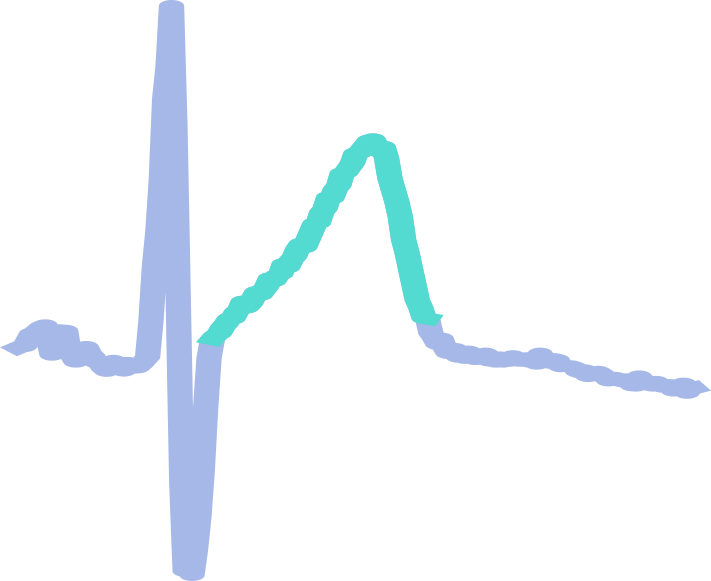
\includegraphics[height=3.5ex, valign=m]{large_peak_ecg.png}) or "\textit{I am searching for the QRS complex, that looks like a} \texttt{sharp peak followed by a sharp valley} (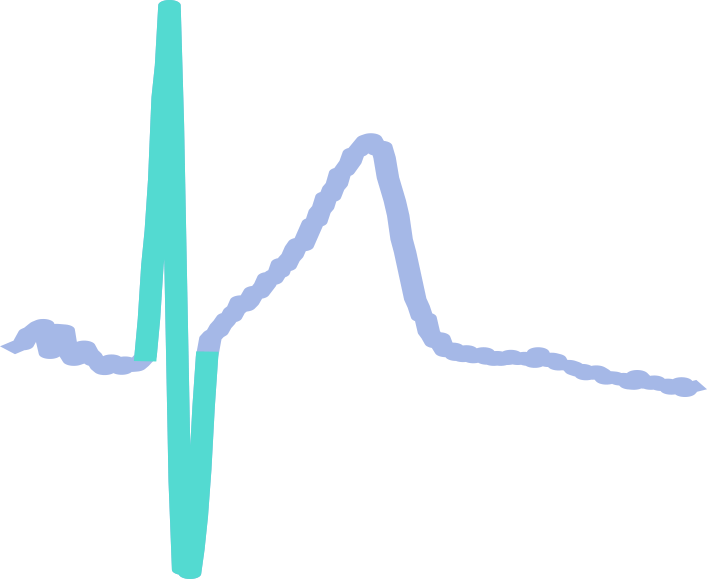
\includegraphics[height=3.5ex, valign=m]{high_peak_ecg.png})". From this textual description of patterns, the reader can associate words with specific properties, such as \texttt{peak} can be related with \textit{slope} and \texttt{high} related with \textit{amplitude}.
\par
The text mining domain already has several approaches to search for specific patterns based on text queries. The reader may already have used the command \textit{cntrl+f} to search for specific words, or used regular expressions to search for specific patterns of words in text documents. Most probably, the reader also uses the \textit{Google Search} toolbar with a simple list of keywords, sorting the list of documents according to these.
\par
In this chapter, we intend to present the reader with solutions that promote a higher flexibility, cognitive-speed and expressiveness in searching for patterns in time series as we typically do with text. Two main strategies were explored: (1) \gls{SSTS} and (2) \gls{QuoTS}. The first profits of a symbolic characterization of the signal, introducing a novel representation and the usage of \textit{regular expressions} to search for patterns on this representation. The second uses a feature based representation of the signal, being each feature attributed to one word, which can be used with additional \textit{operators} to search for the desired patterns with natural language. 
\par
The chapter will start by detailing how \gls{SSTS} works, showing its usage in several examples. In addition, a symbolic representation of the time series can also be used to differentiate classes of signals. Therefore, a proposed strategy towards interpretable time series classification with \gls{SSTS} is introduced and explained as well. This chapter ends with \gls{QuoTS} and how a user can \textit{"google"} patterns on time series with keywords.




%In terms of morphology, many attributes can be extracted from the visual perception of the signal, such as rising and falling slopes, concavity, direction, amplitude thresholding, frequency, time and amplitude range of a slope, among others. For instance, we can identify positive peaks by finding a rising slope followed by a falling slope, which is precisely the mechanism developed in Horowitz \textit{et. al.} for peak detection in electrocardiography~\citep{Horowitz}.
%\par
%We can think of this morphological description in terms of a characterization by means of features. These features can either be used to transform the signal into a symbolic representation, in which each sample is converted to a symbol, or a feature-based representation, in which a \textit{word-feature series} characterizes the time series for a specific property. 
%\par



\section{Syntactic Search on Time Series}

\begin{figure}
\centering
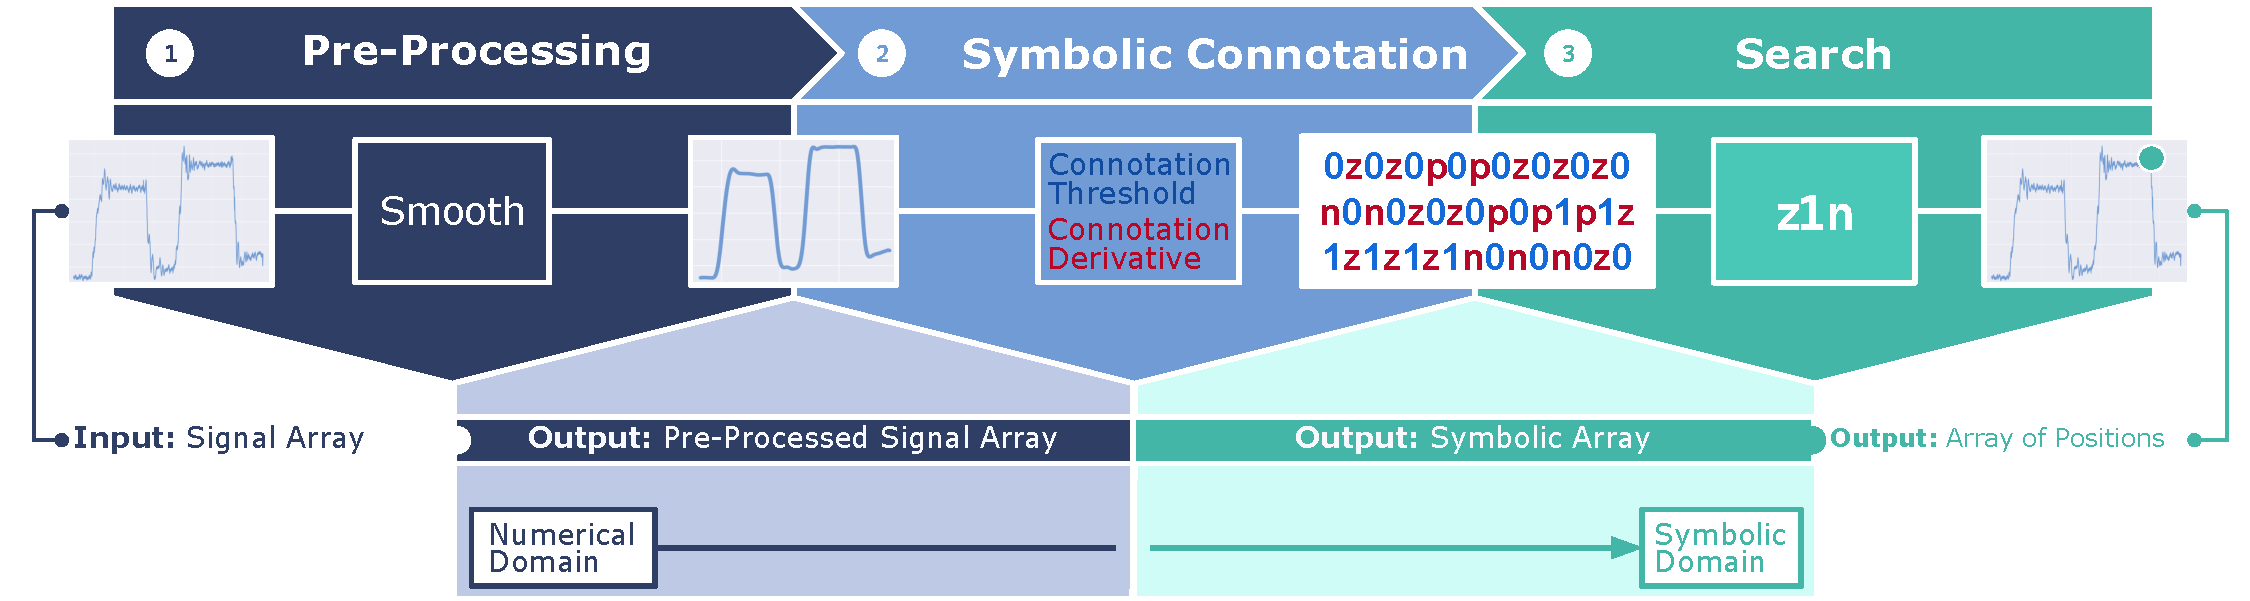
\includegraphics[width=\linewidth]{ssts_intro.pdf}
\label{fig:ssts_intro}
\caption{SSTS modular architecture: the proposed system is divided into three main modules - pre-processing, symbolic connotation and search.}
\end{figure}

In Chapter \ref{cha:theory} was presented the well-known \gls{SAX}, which is a symbolic representation of the time series based on the amplitude distributions. With \gls{SAX}, query with text was not considered, but \gls{SSTS} takes inspiration of this symbolic transformation by including additional attributes besides amplitude, such as the derivative, speed of the derivative, etc.... Each property characterizes each sample of the signal. The combination of these attributes into sequence of primitives is a symbolic characterization of the signal that enables the use of regular expressions for searching the desired pattern. The proposed tool focuses on the knowledge retrieved from the visual interpretation of the signal that enables the search of the desired patterns by writing a regular expression that parses the syntactic representation of the signal.
\par
The proposed tool, \gls{SSTS}, uses symbolic sequences to perform each of the three steps that compose it: \textit{pre-processing} - prepare the signal to highlight the desired patterns and ease the search process; \textit{connotation} - symbolic representation of time series into a set of primitives that give information about the shape and attributes of the time series over time and is governed by a set of grammatical rules; and \textit{search} - a parser (\gls{regex}) to search for patterns in the symbolic representation. Both \textit{pre-processing} and \textit{connotation} steps rely on \textit{tokens} to call specific methods.
\par
The next sections explain each step of the \gls{SSTS} process and will be accompanied by an example to elucidate how it works. The represented signal is the \textit{z} axis of an accelerometer placed in the wrist of a subject while performing a rotating task in different angles. The purpose of this example is to find the time intervals where the plateaus above a certain threshold begin to decrease. Each step of this problem's resolution is shown in Figure \ref{fig:Exercise1} and will be thoroughly explained throughout the next sections. We take the liberty to start introducing some of the processing tokens ( $Sm$ is the smooth function, $A$ is the Connotation Threshold and $D1$ is the Connotation Derivative) to give a base complete example of the usage of the \gls{SSTS}.


\subsection{Pre-Processing - Preparing the Data}

The pre-processing stage is responsible for preparing the signal, either by removing noise that arises from several sources or adjusting the signal so that the information is unveiled. Traditional pre-processing methods, such as a pipeline of linear filters, moving window average filters and statistical de-noising or re-sampling techniques, are typical procedures to prepare the signal for further tasks \cite{preProcessing}. The current approach uses a symbolic representation of these techniques, in which each is represented by its corresponding \textit{token}, which can be a symbol or a function name. In order to manage the pre-processing tasks, a string containing a set of tokens and their corresponding arguments is written by following the polish notation \cite{polishNotation}, in which the token precedes the corresponding argument(s), and each element is separated by a white-space character. The available pre-processing methods to be used with \gls{SSTS} are presented in Table \ref{tab:preprocess}.
\par
In the example of Figure \ref{fig:ssts_intro}, the pre-processing step uses the following string: "$Sm$ 500", which indicates that a smooth filter using a window with a size of 500 samples is applied to the signal. The resulting signal is showed under the original one. The area sectioned in the plots represents the segment of the signal that will be represented in subsection \ref{subsec:symbolic_connotation}.

\begin{center}
\begin{table}
	\centering
    \setlength{\tabcolsep}{3pt}
	\renewcommand{\arraystretch}{1.5}
	\caption{List of common \gls{SSTS} pre-processing operators. As input parameters, \textit{s} is the signal, \textit{fc} is the cut-off frequency and \textit{win\_size} is the size of the window used (number of samples). The linear filters (HP, BP and LP) have a default order of 2}
	~\\~
	\label{tab:preprocess}
	\begin{tabular}{lcL{0.7\linewidth}}
        \toprule[0.5mm]
		Name & Input Parameters & Description\\
        \midrule[0.3mm]
		HP & (\textit{fc}) & Linear high-pass filter with cut-off frequency \textit{fc}\\
        \midrule
		BP & (\textit{fc1}, \textit{fc2}) & Linear band-pass filter with cut-off frequencies \textit{fc1} and \textit{fc2}\\ 
        \midrule
 		LP & (\textit{fc}) & Linear low-pass filter with cut-off frequency \textit{fc}\\
        \midrule
        abs & none & Modulus of signal - $|T|$\\
        \midrule
        Mag & none & Magnitude - $|T| = \sqrt[]{T_0^2 + T_1^2 + T_2^2}$\\
        \midrule
        Sm &  (\textit{win\_size}) & smoothing of \textit{T} by a moving average window filtering technique of size \textit{win\_size}\\
        \midrule
        Z_{norm} & (\textit{s}) & z-normalize the time series $\overline{T} = \frac{T-\bar{\mu_T}}{\sigma_T}$, being: $\overline{T}$ the normalized signal, $\bar{\mu_T}$ the signal's mean and $\sigma_T$ the standard deviation of the signal\\
        \midrule
        | & N.A. & Separates the pre-processing methods applied to multiple signals or multiple processing of the same signal\\
        \bottomrule[0.5mm]
 	\hline
	\end{tabular}
\end{table}
\end{center}

\subsection{Connotation - The Symbolic Time Series}
\label{subsec:symbolic_connotation}


\begin{figure}
\centering
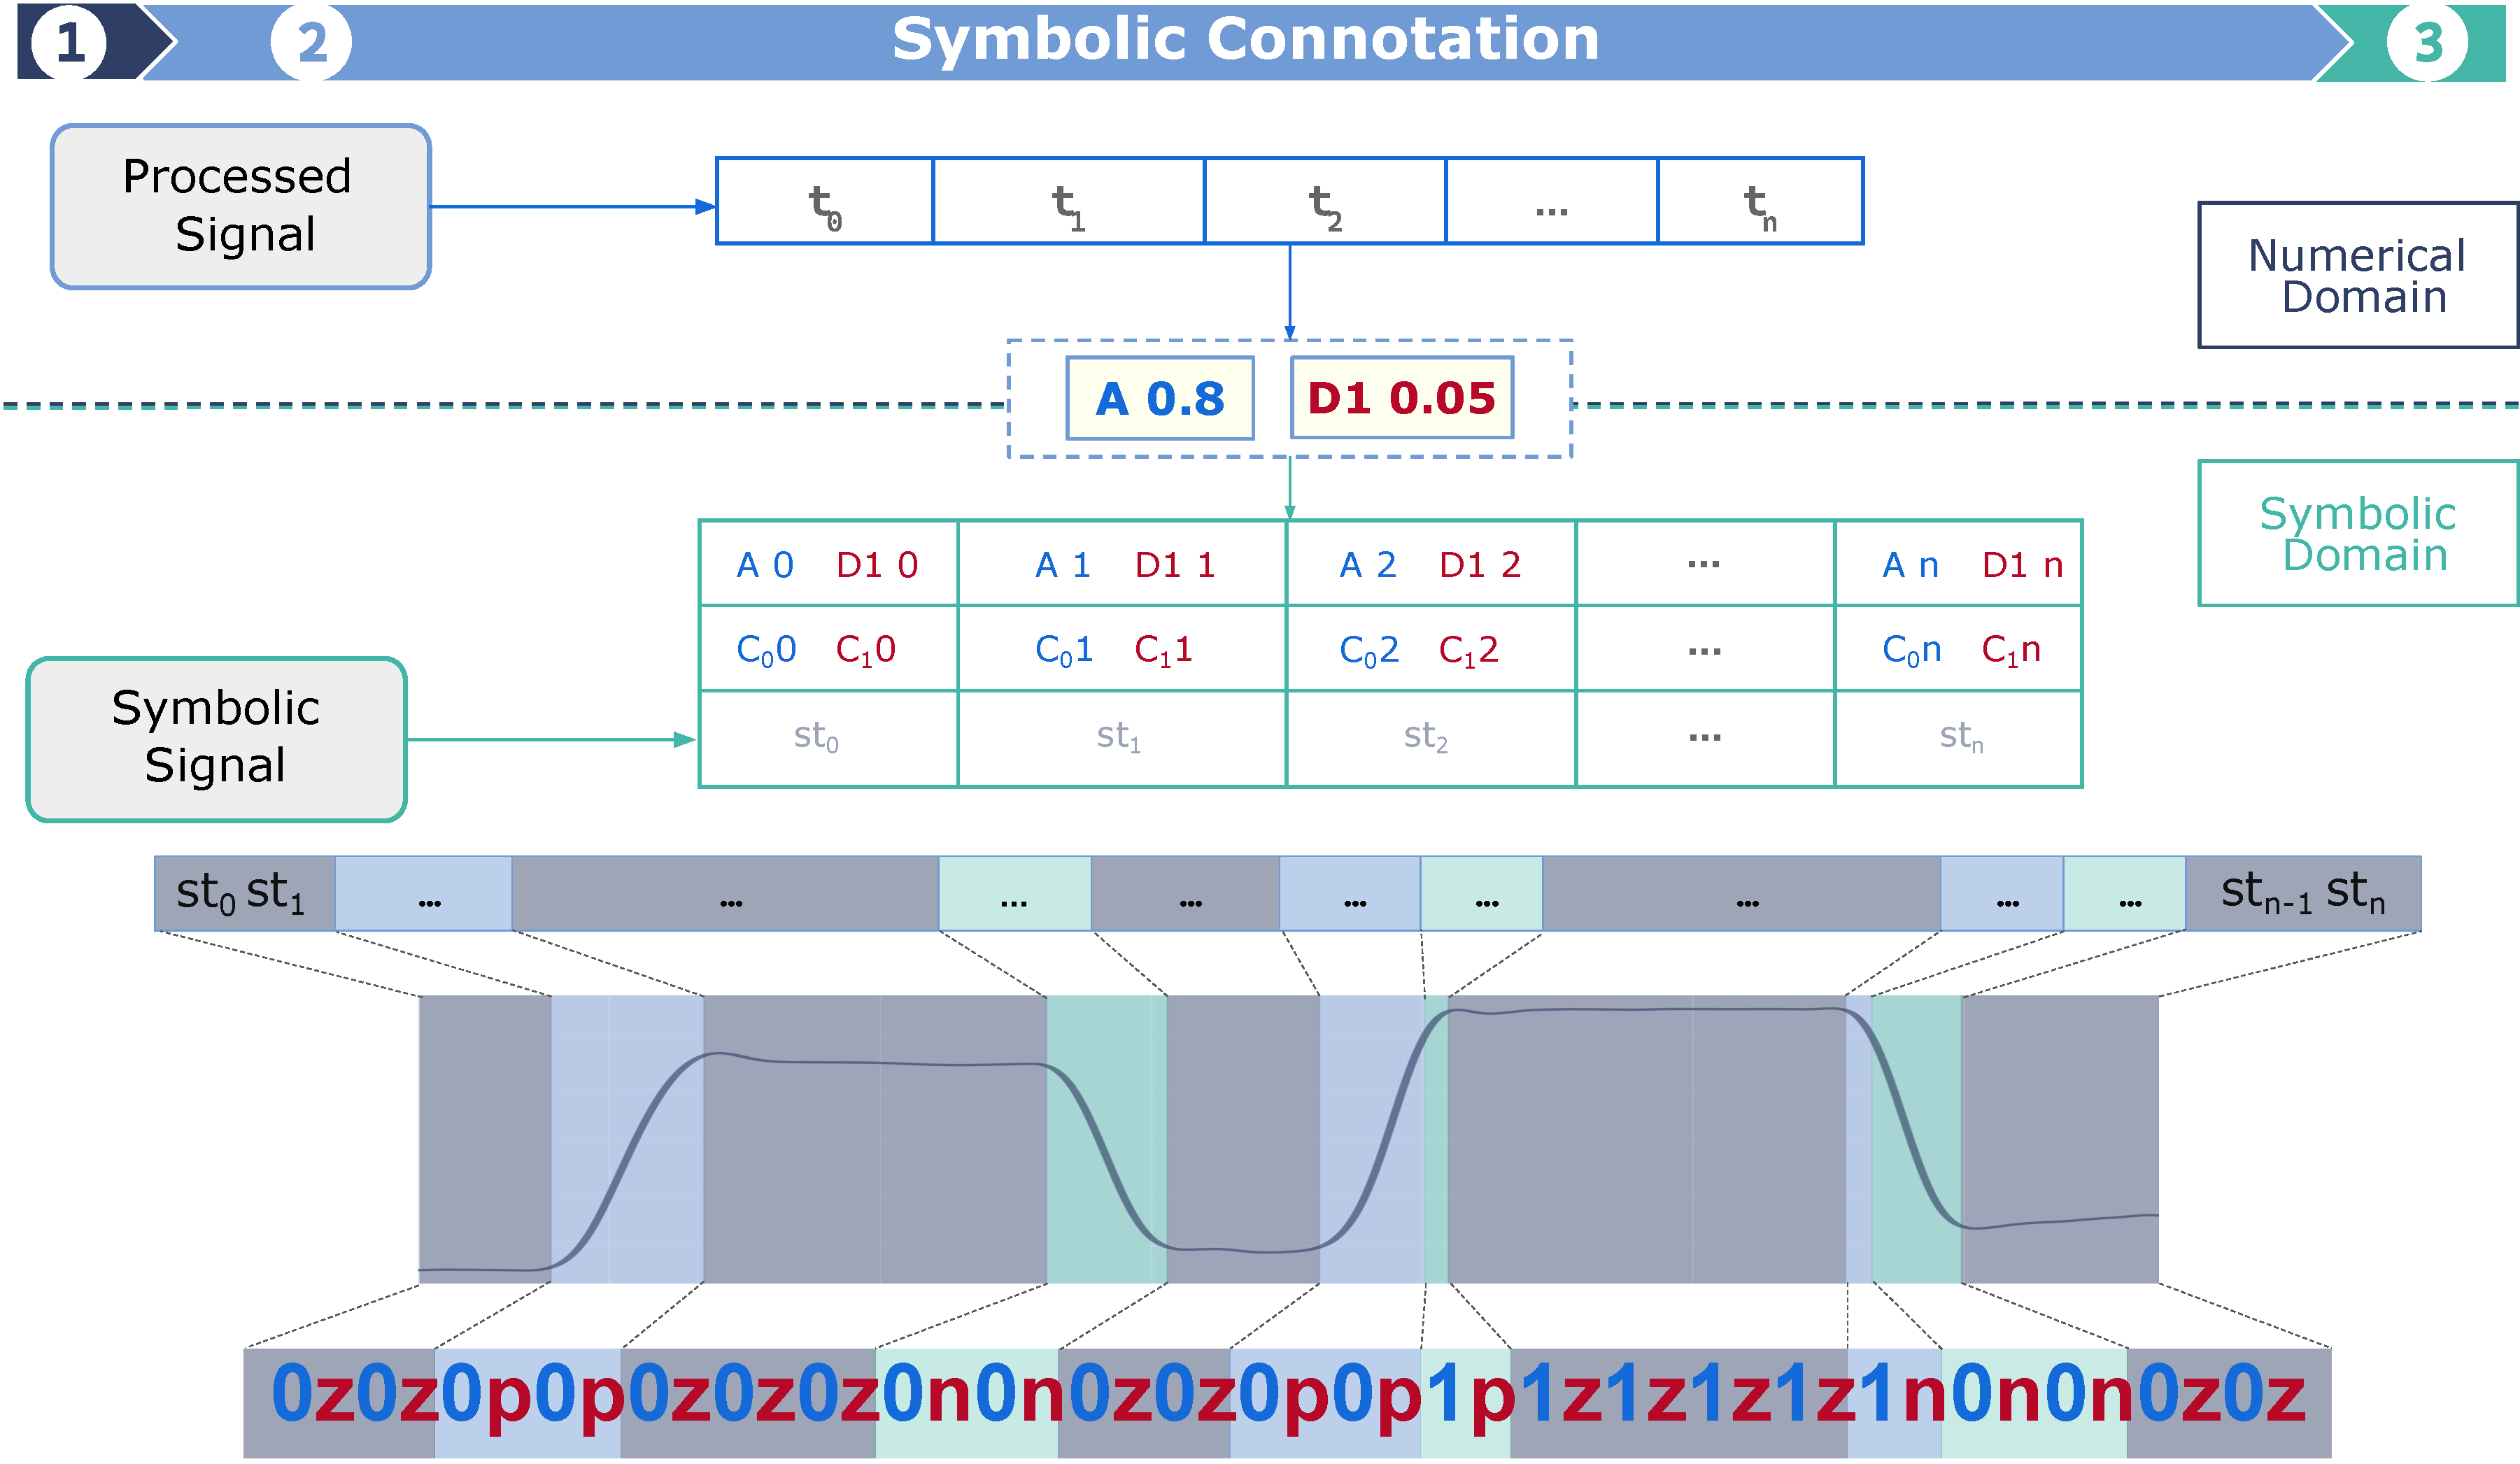
\includegraphics[width=\linewidth]{ssts_connotation_step.pdf}
\label{fig:ssts_intro}
\caption{SSTS modular architecture: the proposed system is divided into three main modules - pre-processing, symbolic connotation and search.}
\end{figure}

In semiotics, it is described that the connotative aspect of an image or a sign corresponds to the extraction of meaning (sometimes called the \textit{second meaning}), by the personal interpretation of its traits and characteristics \cite{connotation}. The \textit{connotation}step is exactly the same connotative aspect, but of a time series. In this, the interpreter (the analyst) has made his personal analysis of the time series and retrieved the necessary information in order to search for the desired patterns. 
\par
The symbolic \textit{connotation} step generates a sequence of \textit{characters} by extracting properties of the signal that are based on a conversion rule the user defines. Each of these conversion rules are designated the \textit{connotation} methods and are responsible for converting each sample of the signal into a \textit{character} or group of \textit{characters} that represent the state of the sample for that conversion rule. Each of the \textit{connotation} methods is related with specific attributes of the time series that are considered relevant for the search procedure. The string that results from this step is therefore a symbolic representation of the strictly necessary attributes of the signal that are best suited to specify a pattern match. Note that this process is decided by the analyst.
\par
The string can be based on a single connotation method, or the combination of multiple ones. In addition, the \textit{connotation} process also handles multidimensional signals, in which cases the string is a combination of \textit{connotation} methods corresponding to each time series, returning a group of \textit{characters} for each sample of the time series.
\par
The reader may appreciate that we recall the general text definitions from Chapter \ref{cha:intro}, and associate these with \textit{connotation} step's output. Each sample of the time series, $T=(t_1, t_2, ..., t_n)$,  is converted into a \textit{character} from this \textit{connotation} alphabet ($char_C$), generating a symbolic time series, $ST = (st_1, st_2, ..., st_i, ..., st_n)$, in which $st_i = char_C$. A \textit{character} is any unit symbol from the connotation alphabet ("Group of Symbols" in Table \ref{tab:connotation}). When the analyst selects more than one \textit{connotation} method to transform the time series $T$, each sample of $T$ is converted into the corresponding \textit{characters}, one for each alphabet of each \textit{connotation} method applied, resulting in: $st_i =$ \bnfpn{$char_{C1}$}\bnfpn{$char_{C2}$}\bnfpn{...}\bnfpn{$char_{Cc}$} , being $ char_{Cc}$ the $c^{th}$ \textit{connotation} method applied. In case $T$ is a multi-dimensional time series, the symbolic time series (MST)' samples from each time series are grouped $MST =$ (\bnfpn{$st_{1,1}$}\bnfpn{$...$}\bnfpn{$st_{1,k}$}$,..., $\bnfpn{$st_{n,1}$}\bnfpn{$...$}\bnfpn{$st_{n,k}$}).
\par
The set of connotation methods can be defined by the user and added as needed. A base list of connotation methods and the corresponding symbols used for the examples presented in the paper are listed in Table \ref{tab:connotation}.

\begin{table}[h!]
	\centering
	\caption{List of base \gls{SSTS} connotation operators. The input parameters are \textit{s}, which represents the input signal and \textit{thr}, which defines the threshold percentage value of the amplitude range of the signal ($max(s) - min(s)$) for a given connotation method. The operator that separates the connotation methods applied to multiple signals or multiple representations of the same signal is the vertical bar "\textbf{|}".}
	~\\~
	\label{tab:connotation}
   \setlength{\tabcolsep}{3pt}
   \renewcommand{\arraystretch}{1.5}
   \begin{tabular}{
   c M{0.1\linewidth} M{0.2\linewidth} L{0.6\linewidth}} \toprule[0.5mm]
		Name & Input Parameters & Group of Symbols & Description\\ \midrule[0.3mm]
		 A & (\textit{s}, \textit{thr}) & ["1","0"] & Amplitude comparison, If $t_i$ > \textit{thr}*($t_{max} - t_{min}$), $t_i$ is "1", else $t_i$ is "0"\\ 
         
         \midrule
         
		D1 & (\textit{s}, \textit{thr}) & ["p", "n", "z"] & Derivative of signal \textit{s} (\textit{s'}). If $t'_i$ > \textit{thr}, $t'_i$ is 'p'; elif $t'_i$ < \textit{- thr}, $t'_i$ is'n'; else, $t'_i$ is "z". \\ 
        
        \midrule
        
        D2 & (\textit{T}, \textit{thr}) & ["D", "C", "z"] & Second derivative of signal \textit{T} (\textit{T"}). If $t"_i$ > \textit{thr}, $t"_i$ is 'D'; elif $t"_i$ < \textit{- thr}, $t"_i$ is 'C'; else, $t"_i$ is "z". \\ 
        
        \midrule
        
 		AD & (\textit{s}, \textit{thr}) & ["1", "0"] & Determinates if amplitude from a minimum to a maximum and vice-versa is superior to \textit{thr}. If so, $t_i$ is "1", else, $t_i$ is "0". \\  
 		
 		\midrule
 		
 		SA & (\textit{s}, \textit{thr}) & ["r", "R", "f", "F"] & Amplitude of a slope segment. The characters are case sensitive, being \textbf{\textit{r}} for a low rise and \textit{\textbf{R}} for a high rise. The same for falling (\textbf{\textit{F}} or \textbf{\textit{f}}). \\
 		
 		\midrule
 		
 		SS & (\textit{s}, \textit{thr}) & ["r", "R", "f", "F"] & Speed of the signal measured by the amplitude on the first derivative. When the sample is quicker than the threshold it is converted to "R" - quick rise or "F" - quick fall, whereas when slower it is converted to "r" - slow rise or "f" - slow fall.\\
        \bottomrule[0.5mm]
	\end{tabular}
\end{table}


The symbolic connotation step of the exercise of Figure \ref{fig:Exercise1} demonstrates the latter formalism. In Figure \ref{fig:Ex_part2}, the processed signal is decomposed in a symbolic sequence by two connotation methods: amplitude (blue) and derivative (red). The first implies that the sample values superior to the threshold \textit{\textbf{0.8}} will be "1", while the rest turns "0", whereas the second gives the value "p" when the signal is increasing, "n" when decreasing and "z" when stationary with a threshold of \textit{\textbf{0.05}}. Each of the samples of the signal is converted into the primitive ($st_1...st_n$) which is the alternate association of the two connotation methods. The approximate result is illustrated by the bottom string, in which can be seen the alternation property and what it translates. The representation made by means of these two methods is expected to be the necessary to ease the search procedure.

\subsection{Expressive Syntactic Search}

\begin{figure}
\centering
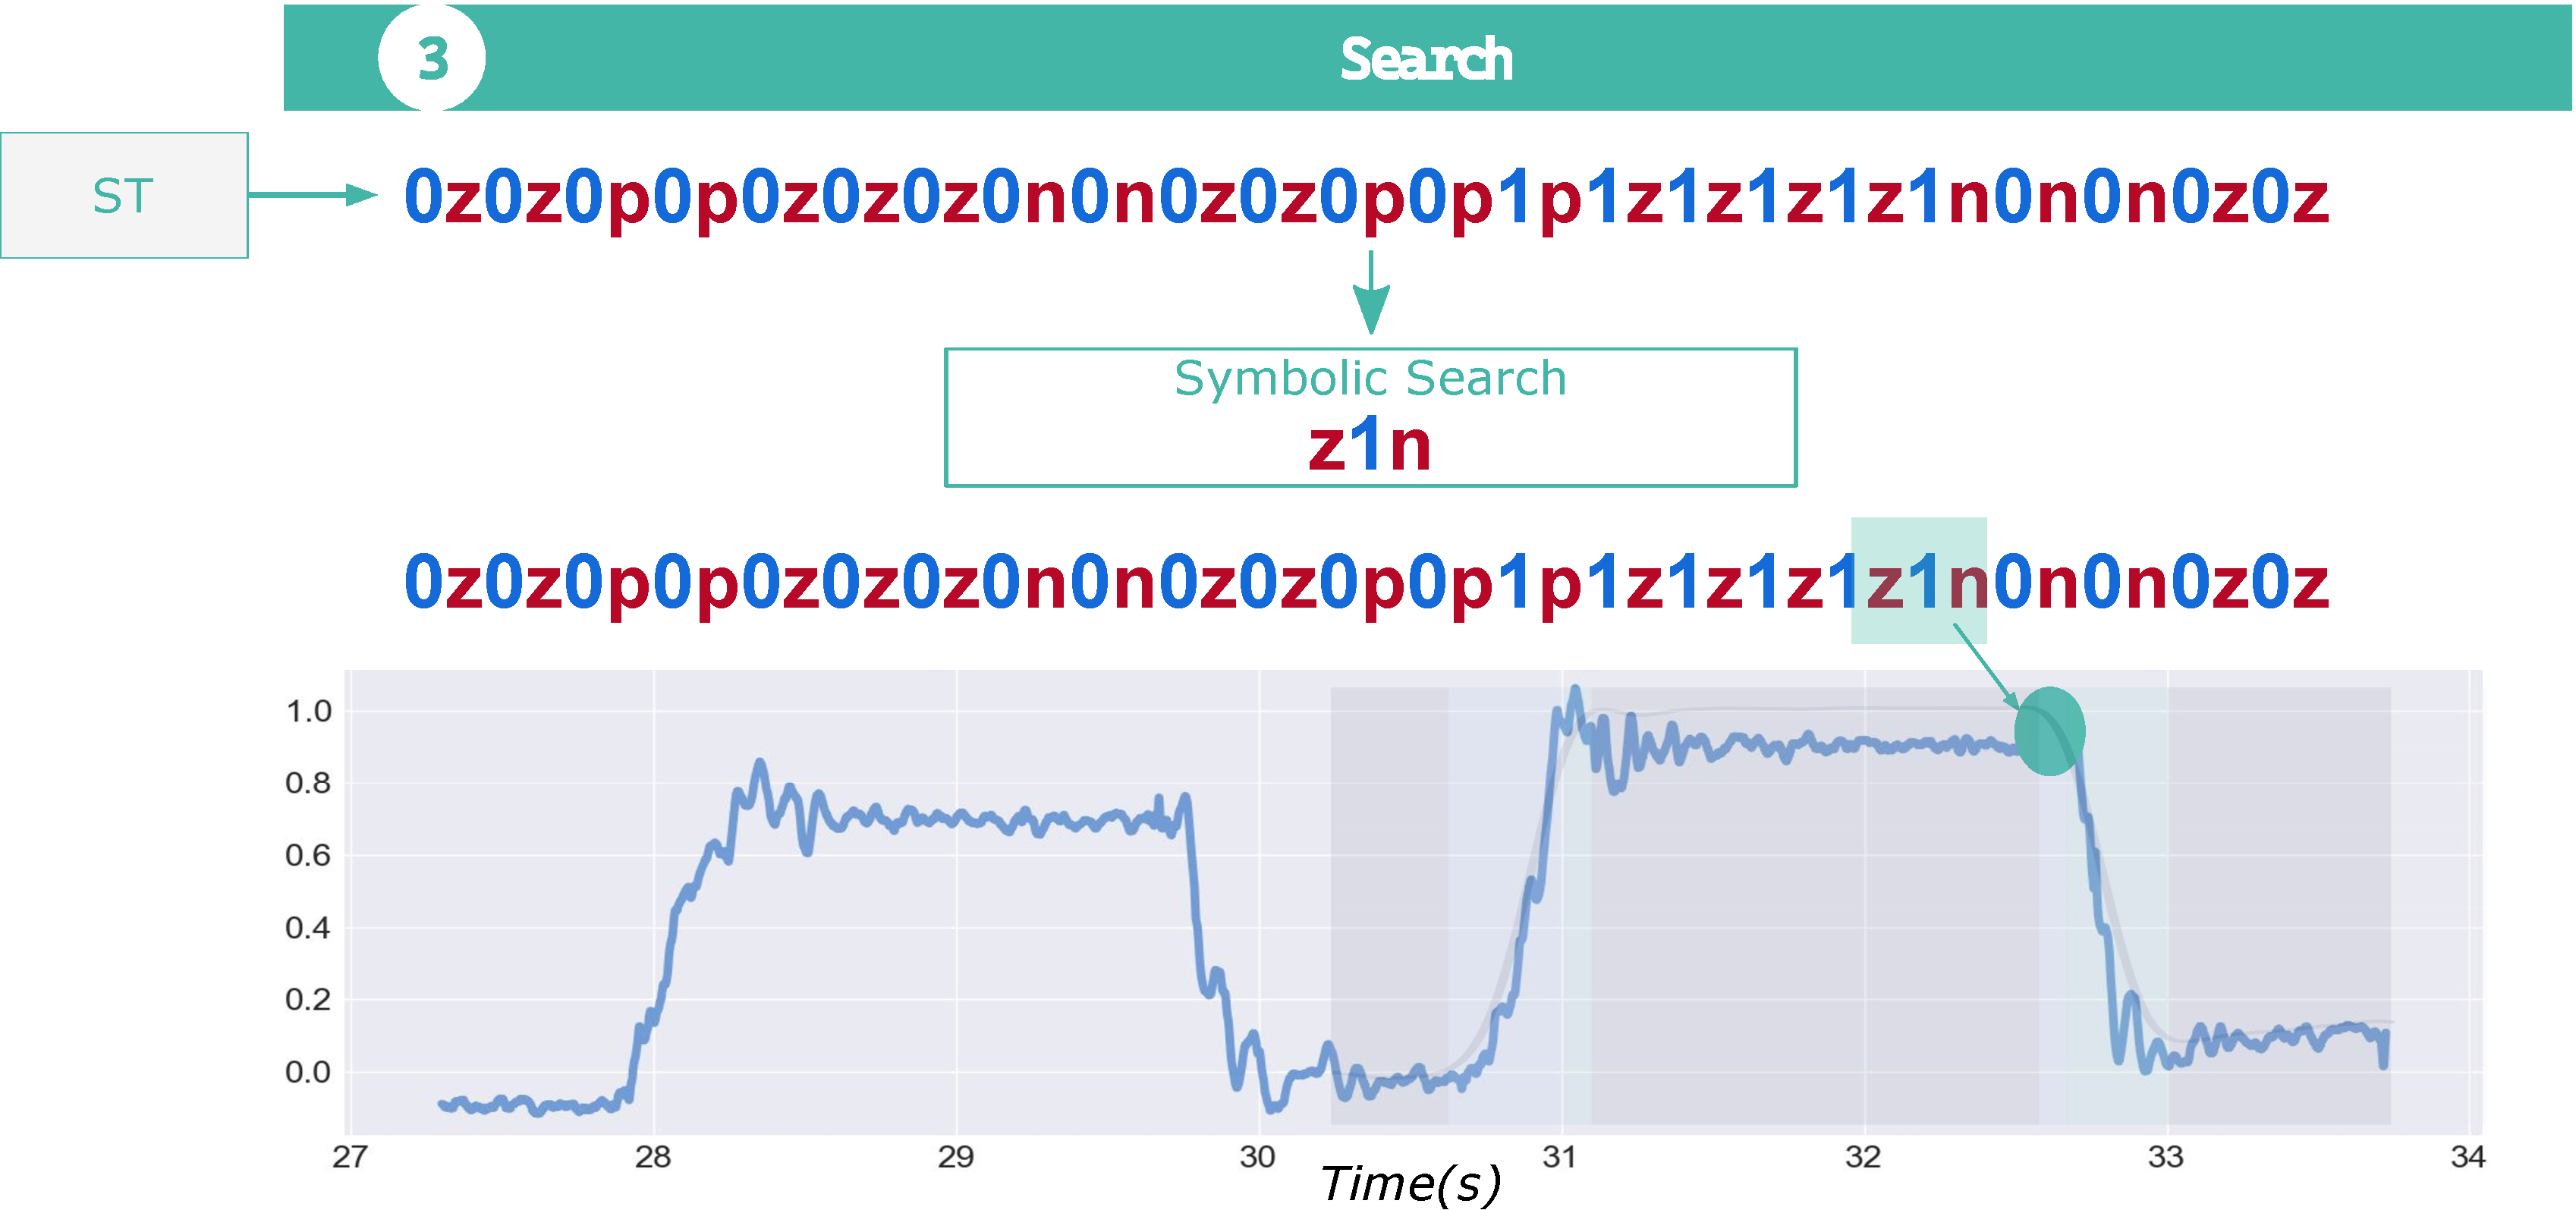
\includegraphics[width=\linewidth]{ssts_search_step.pdf}
\label{fig:ssts_intro}
\caption{SSTS modular architecture: the proposed system is divided into three main modules - pre-processing, symbolic connotation and search.}
\end{figure}

The last step of the process involves searching for the desired pattern in the generated symbolic time series with a regular expression. This string is governed by the rules of regular expressions from the \textit{alternative regular expression Python module} \cite{rgxPy} and benefits from all the functionalities and meta-characters typically used with this tool, which can be recalled from Chapter \ref{cha:theory}.The search procedure returns the intervals at which positive matches occurred. It is relevant to note that it has been decided to use \gls{regex}, although any other parser, conveniently combined with the previous steps, might be used for the same purpose.
\par
In the example of Figure \ref{fig:Exercise1}, the purpose is to determinate when a plateau superior to \textit{80 \%} of the amplitude range of the signal starts to fall, which based on the string representation of the second step is indicated by a "1" and a sequence of stationary ("z") to falling ("n"). The regular expression used for the search is precisely \textit{z1n}, which indicates that the signal, at some point superior to the threshold will start to decrease. 
\par
In Figure \ref{fig:Ex_part3} is presented this reasoning.
The next chapters will provide some examples, based on real data, in which each of the steps will be thoroughly explained in order to fully understand the capabilities of the \gls{SSTS} tool.








In this study, we propose a tool that focuses in ease simple query search tasks in time series, which we refer as \gls{SSTS}. This is achieved by an innovative methodology, where the user gives a syntactic nature to time series, which turns the search procedure less verbose and more related with the reasoning of the user in recognizing the desired pattern.







\section{Towards Interpretable Time Series Classification with SSTS}

\begin{figure}
\centering
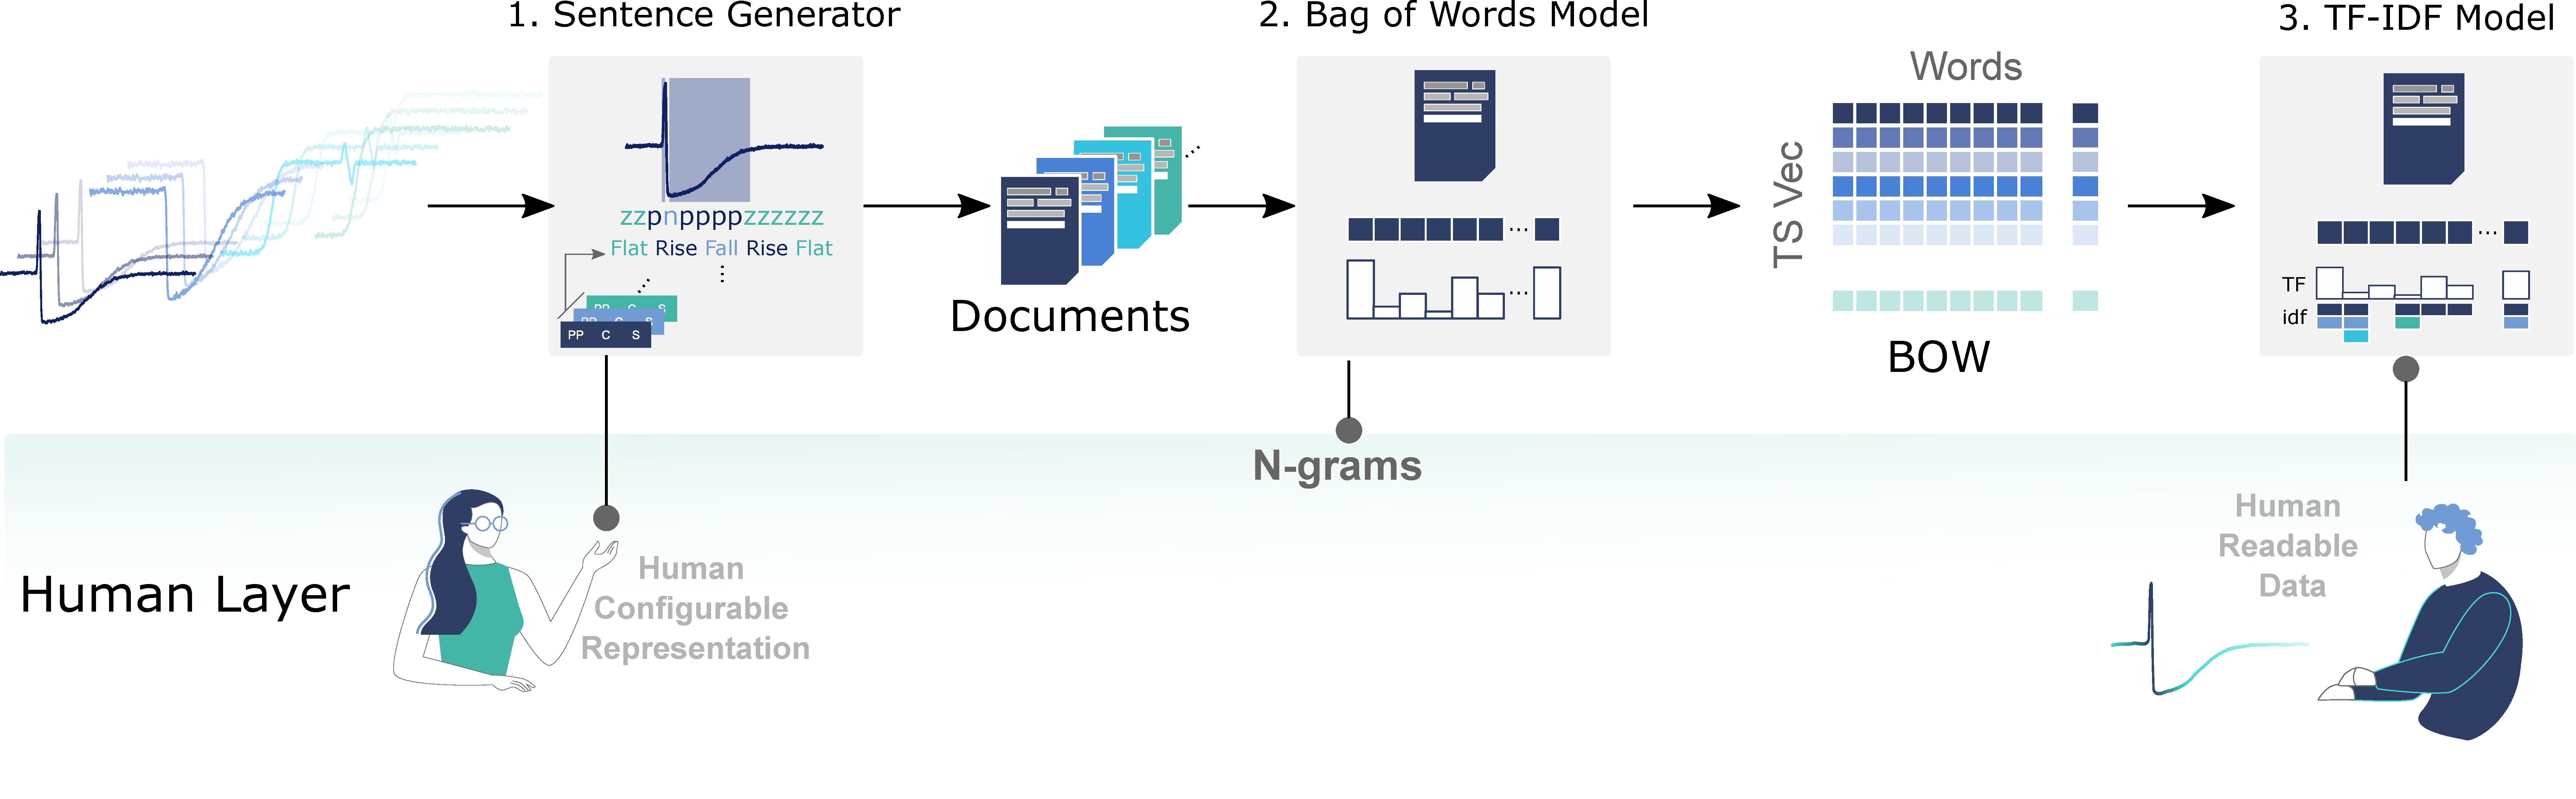
\includegraphics[width=\linewidth]{overall_interpretable.pdf}
\label{fig:ssts_intro}
\caption{SSTS modular architecture: the proposed system is divided into three main modules - pre-processing, symbolic connotation and search.}
\end{figure}


The ability to transform a time series into a meaningful symbolic representation makes the usage of text mining tools available for time series analysis. This means that the analysis process can be different and complement traditional methods or even bring novel strategies by thinking in how to solve it differently. What is proposed in this section is to use this novel representation to profit from the text mining knowledge and use it into time series classification. In order to perform a class separation, differences and similarities have to be highlighted, and this is also possible to be done with text.
\par
In text mining, the difference between text \textit{documents} is traditionally performed with a feature extraction process on text, such as \gls{bow} or \gls{tfidf}, returning a statistical representation of the words or \gls{ngrams}. \textit{Documents} with different words and sequences of words will have different weights on these models, which is used to perform a class separation on the \textit{documents}. In this work, we take inspiration on this process and apply it to time series. Figure \ref{fig:overall_interpretable} shows the main steps to perform a transformation of the time series into a \gls{bow}/\gls{tfidf} model that can be used with a classifier. 
\par
In this section we explain each step of the proposed strategy to perform time series classification based on a textual description with \gls{SSTS}. The fact that the time series are translated into text also provides a layer of readability and interpretability on the data, as we will explore throughout this section.

%
%The proposed method, conceptually developed based on text mining techniques, abstracts how a time series can be structured in a linguistic representation, similar to how the human would describe a time series with words. In order to introduce the reader with this abstraction and representation, we explain how we use \textit{SSTS} to make this abstraction.
%
%
%
%The transcription results in sequences of \textit{characters}. Specific \textit{characters} sequences are translated into \textit{words}.\\
%
%\textit{\textbf{Definition 2.5}} A \textit{word} is a sequence of \textit{characters}. \textit{SSTS} has the \textbf{search} step which provides a way of extracting specific patterns with regular expression queries. We pre-defined a set of search queries that correspond to specific words, such as \textit{rise}, \textit{fall}, \textit{peak}, \textit{valley}, etc.... These words can be associated with a single character (e.g. rise = \textbf{\textit{p+}}) or a combination of them (e.g. peak = \textbf{\textit{p+[z]n+}}). Examples of common matches are presented in Figure.
%
%This set of words belong to a \textit{vocabulary}.\\
%
%\textit{\textbf{Definition 2.6}} The \textit{vocabulary} comprehends the set of words available in a pre-defined set of \textit{SSTS} queries.
%
%The \textit{words} used can be ordered to form a \textit{sentence}.\\
%
%\textit{\textbf{Definition 2.7}} \space \space A \textit{sentence} is a set of \textit{words} or tokens organized sequentially. In this work we create multiple sentences based on the types of \textit{connotation} methods used to transcribe the time series. In Figure \ref{fig:SSTS_example}.Bottom, a time series is translated into the \textit{sentence} \textbf{\textit{Flat Rise Fall Rise Flat}} based on a set of \textit{SSTS} queries from the derivative connotation (\textit{\textbf{p+, z+}} and \textbf{\textit{n+}}). 
%For each time series, one document is generated. 
%
%\textit{Sentences} can be added to a \textit{document}. \\
%
%\textit{\textbf{Definition 2.8}} \space \space A \textit{document} is a piece of text with a collection of words or tokens that are used to build sentences. It can be made of only one sentence or multiple ones. In this work, a \textit{time series document} will have multiple sentences as groups of describing patterns. 
%Finally, the higher hierarchy in textual information is the \textit{corpus}.\\
%
%\textit{\textbf{Definition 2.9}} \space \space The \textit{corpus} is a collection of text material (group of documents). It represents the higher level of textual information. This collection is typically annotated and used for machine learning tasks. In this case, a corpus will be represented by the set of documents that describe a time series dataset.
%
%Since this work follows the steps of \textit{NLP} strategies for document classification, we will define \textit{Bag of Words} (BoW).\\
%
%\textit{\textbf{Definition 2.10}} \space \space A BoW is a feature matrix representation of a corpus, being the feature the number of occurrences of each word, the term-frequency (\textit{tf}):
%\begin{equation}
%    tf_{t,d} = \frac{f_{t,d}}{\sum\limits_{t'\in d} f_{t',d}}, 
%\end{equation}
%
%being \textit{t} the term that exists in a document, \textit{d} the document, \textit{t'} the term that belongs to document \textit{d}.
%
%We use the BoW to vectorize the textual representation of each time series.
%
%Most of the times, \textit{n-grams} are used in addition to single words.\\
%
%\textit{\textbf{Definition 2.11}} \space \space \textit{N-grams} are a span of followed words that are counted in the BoW. It gives more context to words that are frequently followed by a specific word. As with time series we have temporal order of occurrences, this feature is very important. An example of \textit{2-gram} from the sentence \textit{Rise Flat Fall} would be \textit{Rise Flat} and \textit{Flat Fall}.

\subsection{SSTS to Generate Time Series Documents}



\begin{figure}[!h]
    \centering
    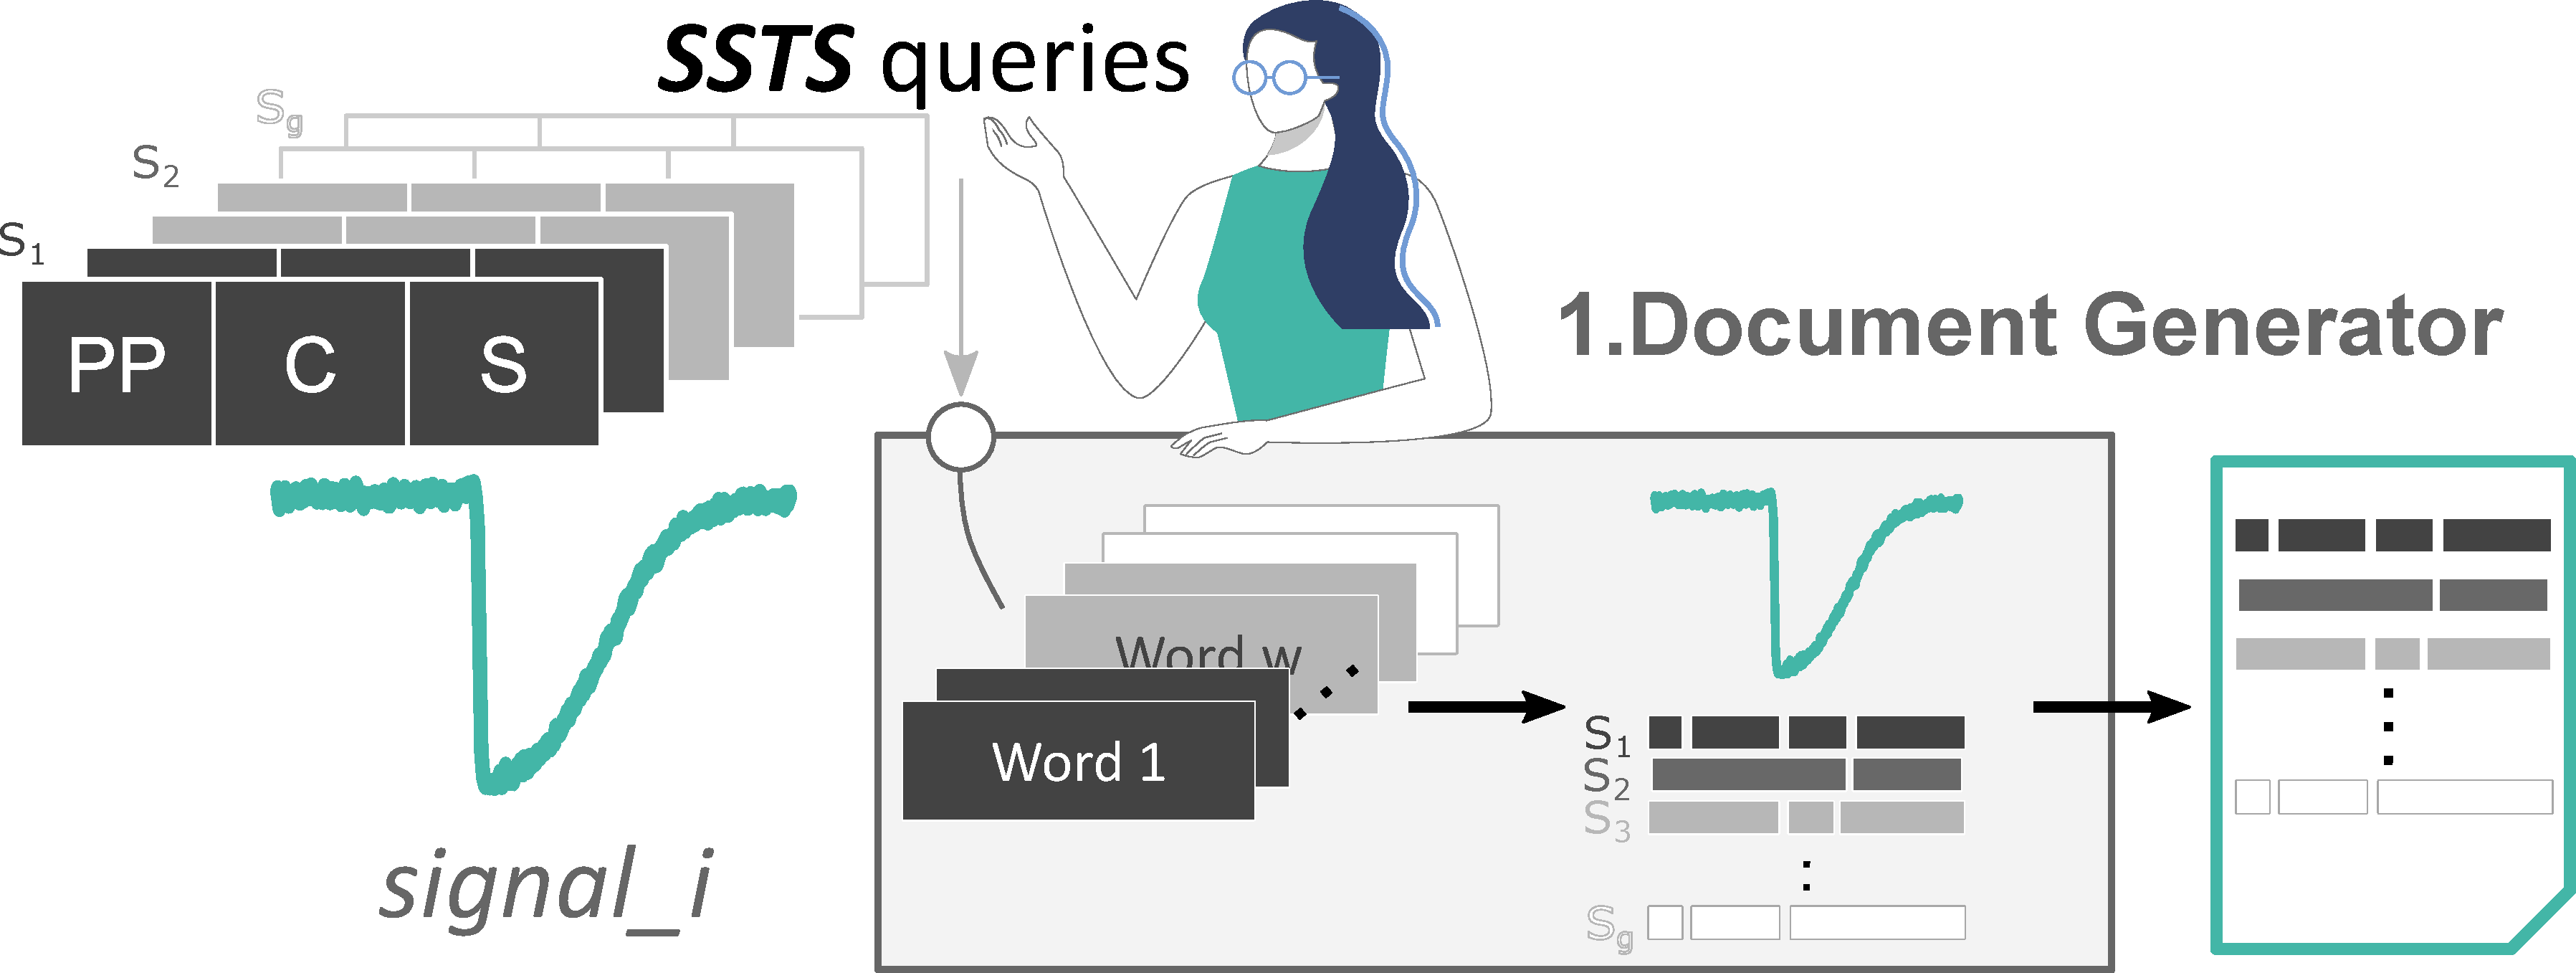
\includegraphics[width=0.85\linewidth]{interpretable_class_intro.pdf}
    \caption{Steps for the generation of sentences from a raw time series and organization as a document. Here: {PP - Pre-processing, C- connotation and S - Search} are each \gls{SSTS} queries used to search for the patterns and attribute the matched \textit{subsequences} the corresponding \textit{word}.}
    \label{fig:sentence_gen}
\end{figure}

Samples of the signal are converted to characters, patterns are searched to form words, and these are ordered by their time index. With this, the time series can be translated into sentences and be described just as a human would describe it. For instance, this signal 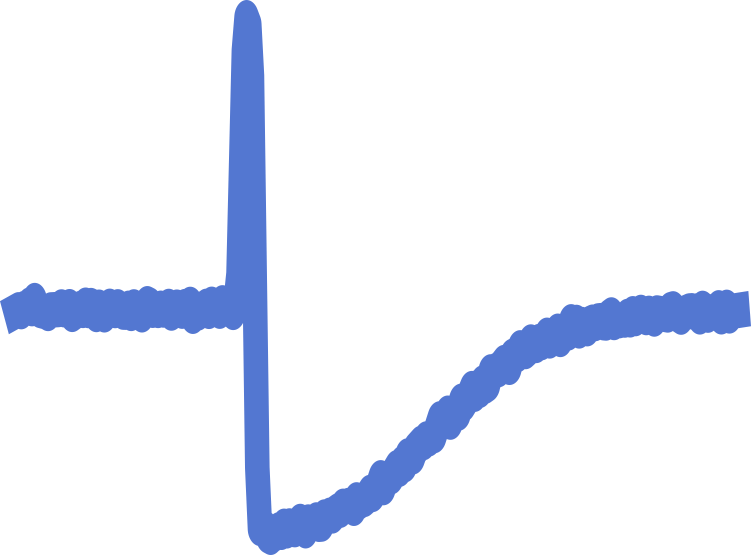
\includegraphics[height=2.5ex, width=3.5ex, valign=m]{trace1.png} can be very broadly translated into \texttt{Flat Rise Fall Rise Flat} or \texttt{Flat Peak Valley Flat}, while this signal 
\includegraphics[height=2.5ex, width=3.5ex, valign=m]{trace_2.png} would be translated into \texttt{Flat Fall Rise Flat} or \texttt{Flat Valley Flat}. This type of description is easily performed with \gls{SSTS}, as showed on Figure \ref{fig:SSTS_example}.
\par
In order to perform this description, the words have to be associated with a specific \textit{\gls{SSTS} query}. Each query is a \gls{regex} pattern that searches the match on the time series and attributes it its corresponding \textit{word}. For instance, the query \{PP: Sm 25, C: D1 0.05, S: p+\} searches for moments where the time series is increasing and attributes to these \textit{subsequences} the word \textit{Rise}. A specific set of \gls{SSTS} queries are used to build a full description of the signal dynamics in higher leveled structures, mostly with amplitude and derivative \textit{connotations}. 
The selection of \gls{SSTS} queries is made by the analyst, either using pre-defined set of queries or creating his/her own, more appropriate for the type of signals to analyze. This is the customizable step of the process, in which the analyst can include his/her intuition.
\par
The ability to distinguish time series with text will be as good as the descriptive richness of the generated sentences. Depending on the differences between the time series being classified, a simple description based on the sign of the signal's derivative might be enough. However, in some cases, the overall dynamic of signals might be dissimilar in other dimensions. In order to have a rich foundation to perform a sentence description of a time series, we created the set of \gls{SSTS} queries presented on Table \ref{tab:ssts_queries}, grouped by sentence ($S1, S2, ...$). 
The table also has an example of matching the corresponding query on a real signal. We would like to highlight that these queries are not mandatory and can be adapted by the analyst or event new connotation methods and queries can be created that might make more sense for the problem being solved. In cases where the user knows exactly what kind of patterns are relevant to perform the distinction, specific patterns can be used, targeting the relevant differences. Otherwise, the existing list can be used.

\begin{table}
\begin{center}
\caption{The connotation variables, search regular expressions and corresponding words assigned to the pattern searched. The parameter \textit{m} indicates the size, in samples, of the difference between a peak or a plateau.}.
\renewcommand{\arraystretch}{1.2}
\begin{tabularx}{\linewidth}{ XXXXX } 
\toprule[1.5pt]
Sentence Group & Connotation & Search & Word & Example\\
\toprule
  \multirow{3}{1em}{S1} & \multirow{3}{3em}{D1 thr} & p+ & \textcolor{mygreen2}{Rising} &  \multirow{3}{9em}{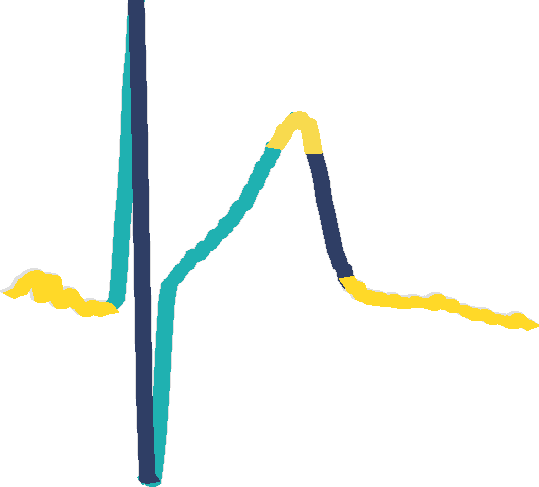
\includegraphics[height=10ex, valign=m]{ecg_overall.pdf}}\\ 
  & & n+ & \textcolor{myblue2}{Falling} & \\ 
  & & z+ & \textcolor{myorange}{Flat} & \\
\hline
 \multirow{4}{1em}{S2} & \multirow{4}{6em}{D1 thr} & p+z\{,m\}n+ & \textcolor{myblue2}{Peak} & \multirow{4}{9em}{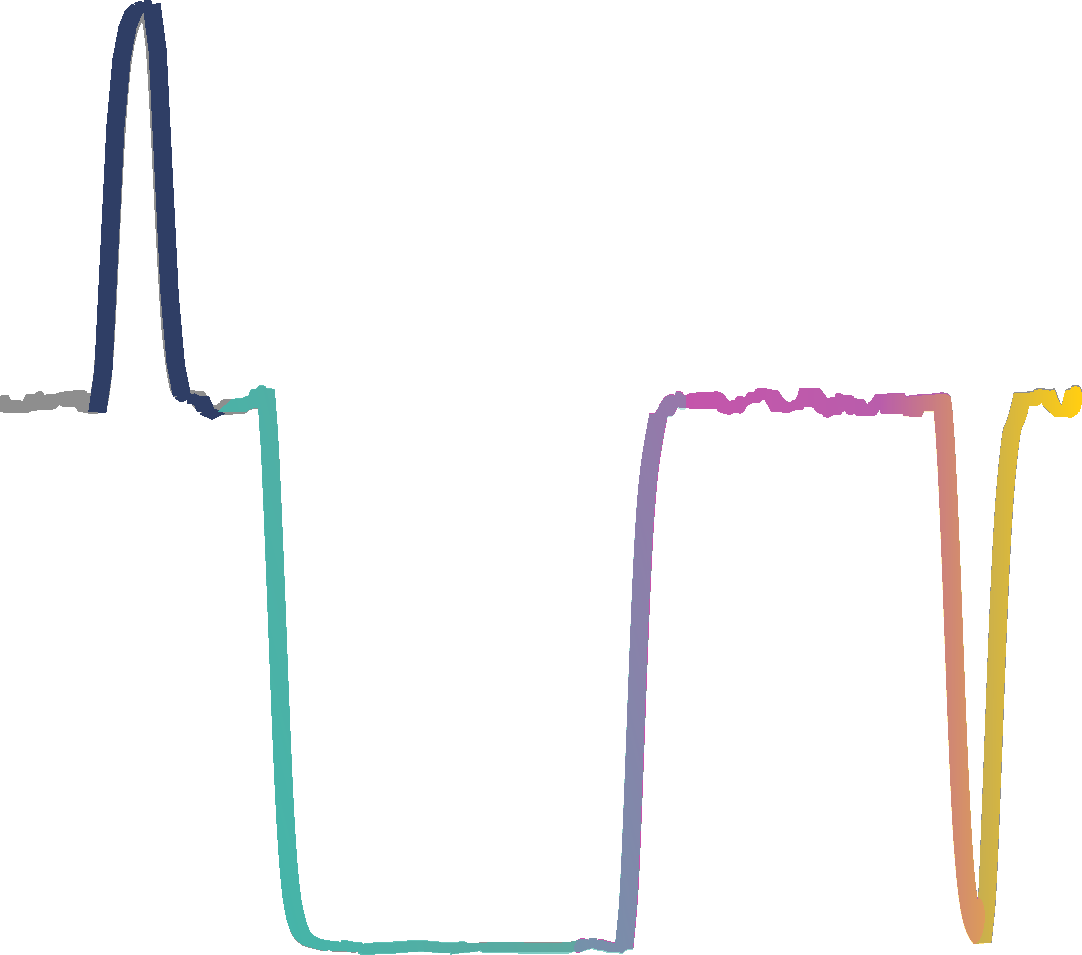
\includegraphics[height=10ex, valign=m]{peak_val_plat.pdf}}\\
 & & n+z\{,m\}p+ & \textcolor{myorange}{Valley}\\
 & & p+z\{m,\}n+ & \textcolor{mypurple}{posPlateau}\\
 & & n+z\{m,\}p+ & \textcolor{mygreen2}{negPlateau}\\
\hline
\multirow{4}{1em}{S3} & \multirow{4}{6em}{SA thr} & r+ & \textcolor{mypurple}{smallRise} & \multirow{4}{9em}{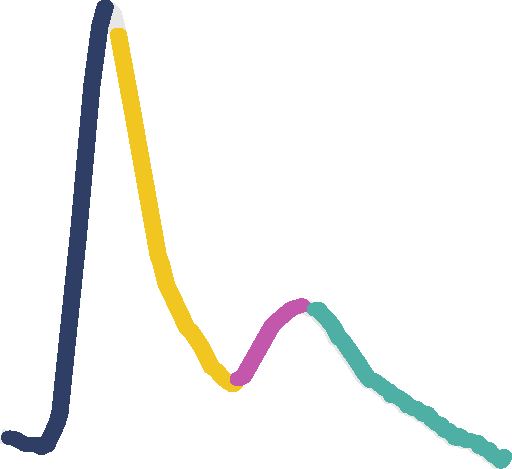
\includegraphics[height=10ex, valign=m]{abp_overall.pdf}}\\
 & & R+ & \textcolor{myblue2}{highRise}\\
 & & f+ & \textcolor{mygreen2}{smallFall}\\
 & & F+ & \textcolor{myorange}{highFall}\\
\hline
\multirow{4}{1em}{S4} & \multirow{4}{6em}{SS thr} & R+ & \textcolor{mygreen2}{quickRise} & \multirow{4}{9em}{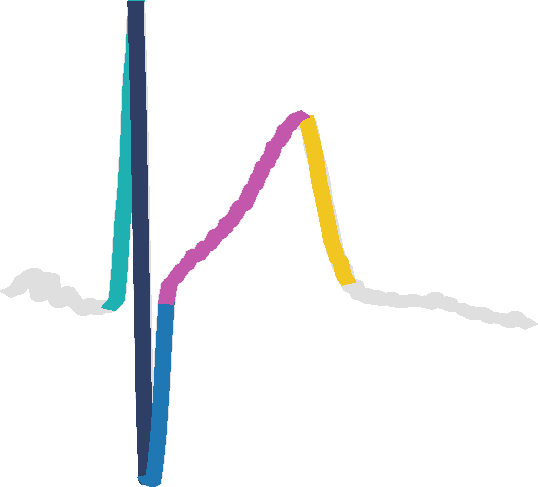
\includegraphics[height=10ex, valign=m]{ecg_overall2.pdf}}\\
  & & r+ & \textcolor{mypurple}{slowRise}\\
  & & F+ & \textcolor{myblue2}{quickFall}\\
 & & r+ & \textcolor{myorange}{slowFall}\\
\hline
\multirow{4}{1em}{S4} & \multirow{4}{6em}{A 0.5 D1 thr} & (0p)+(0z)*(0n)+ & \textcolor{mygreen2}{bottomPeak} & \multirow{4}{9em}{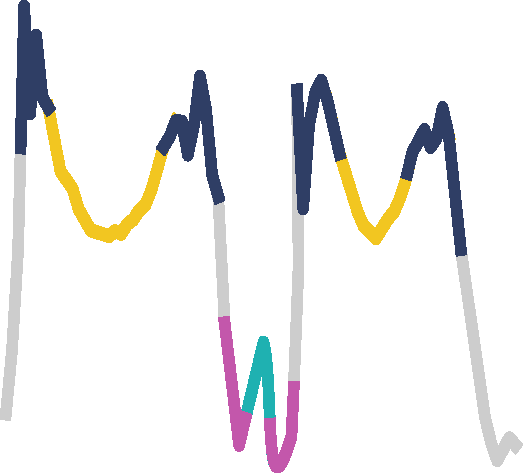
\includegraphics[height=10ex, valign=m]{example_overall_queries_4.pdf}}\\
 & & (1p)+(1z)*(1n)+ & \textcolor{myblue2}{topPeak}\\
 & & (0n)+(0z)*(0p)+ & \textcolor{mypurple}{bottomValley}\\
 & & (1n)+(1z)*(1p)+ & \textcolor{myorange}{topValley}\\
 \hline
\multirow{4}{1em}{S5} & \multirow{4}{6em}{D2 thr D1 thr} & (Dp)+ & concaveRising\\
& & (Dn)+ & concaveFalling\\
& & (Cp)+ & convexRising\\
& &(Cn)+ & convexFalling\\
\bottomrule[1.5pt]
\end{tabularx}
\label{tab:ssts_queries}
\end{center}
\end{table}
 
An example of performing this analysis on a signal is presented on Figure \ref{fig:SSTS_example}. The process highlights the usage of \gls{SSTS} queries from two different groups of sentences. From the first group, the signal is analyzed in terms of derivative, matching parts of the signal where it \textit{rises, falls} or is \textit{flat}. A sentence is generated, describing it as \texttt{Flat Rise Fall Rise Flat}. The same process is done now with the second group of \gls{SSTS} queries, but this time, searching for \textit{peaks, valleys and plateaus}. A sentence is then generated based on the matches: \texttt{Peak Valley}. The same process is applied to each class of signals, being, for each signal, generated a \textit{document} with the corresponding sentences.

\begin{figure}[!h]
    \centering
    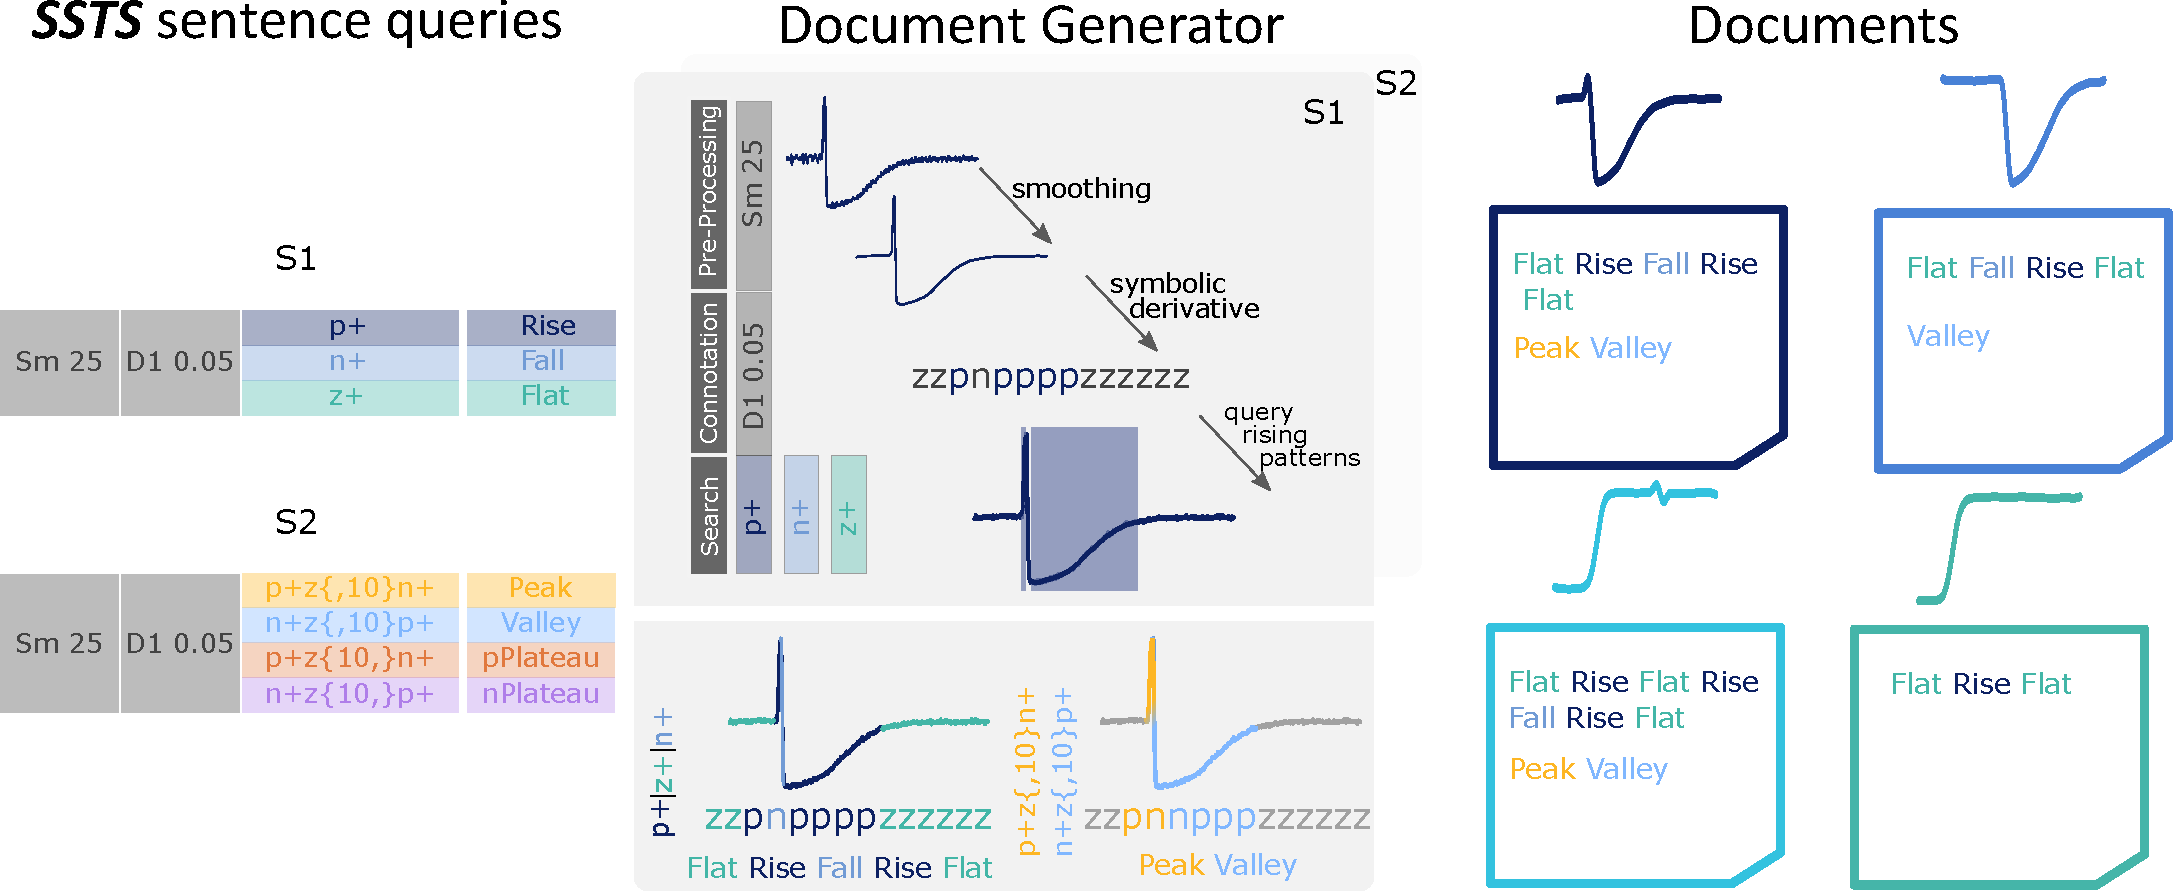
\includegraphics[width=\linewidth]{sentence_generation.pdf}
    \caption{(Top) Using SSTS to detect the rising stage of a time series. Each step of the process is written described as follows: (1) pre-processing: \textit{Sm} is the function \textit{Smooth} with a window size of 25 samples; (2) connotation: \textit{D1}, indicates the first derivate, from which each sample is converted to \textit{z} - Flat, \textit{p} - rising and \textit{n} falling; (3) search - regular expression \textit{p+} searches for all sequences with 1 or more \textit{p} characters. (Bottom) Example of sentence generation. Using the other search queries (\textit{p+, n+, z+}), we can find the derivative patterns and convert it into ordered words.}
    \label{fig:SSTS_example}
\end{figure}

Having now a method to translate time series into text, we are able to use text mining methods directly on the \textit{documents}. Typically, text data is vectorized with the \gls{BOW} or \gls{TFIDF} models. This brings the reader to the second step of the process.

\subsection{Vectorization of Time Series Documents}

The document generation stage receives a time series and transforms it into a \textit{document} with several sentences, descriptive of its shape and dynamics. As mentioned, this transformation is made with \textit{SSTS}, which searches for specific patterns on a symbolic representation of the signal and for which a word is given.  
\par
After converting the time series into \textit{documents}, the text is analyzed to build a matrix of \textit{word} or \textit{n-gram }frequencies, the \gls{BoW} model. In this case, the features extracted are purely statistical, but can provide a relevant measure of differences between documents. Each row of the \gls{BoW} model is a time series \textit{document}, represented by columns that have the number of occurrences of a \textit{word} or \textit{n-gram}. Figure \ref{fig:bow_model} shows the vectorization of a document as one row of the BoW model.

\begin{figure}[!h]
    \centering
    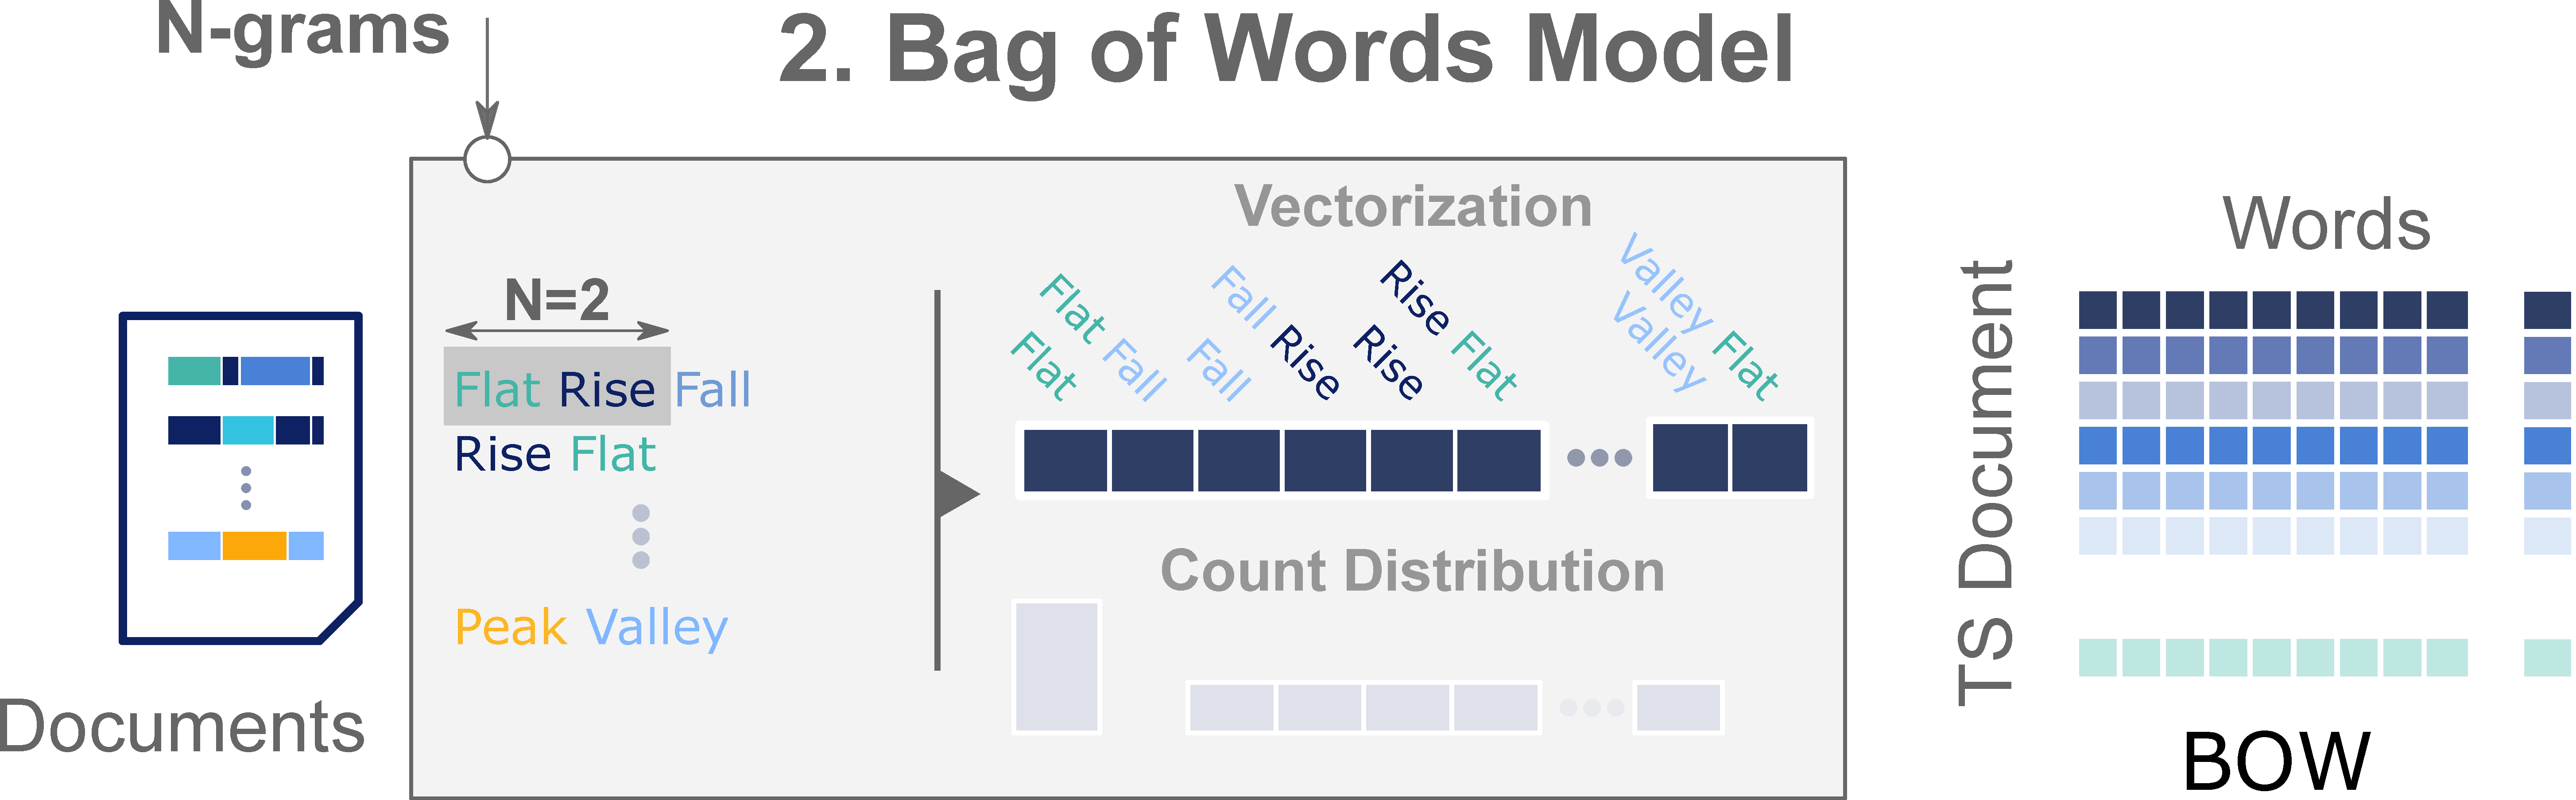
\includegraphics[width=\linewidth]{vectorization.pdf}
    \caption{Steps for the generation of sentences from a raw time series and organization as a document. Here: {PP - Pre-processing, C- connotation and S - Search} are each \gls{SSTS} queries used to search for the patterns and attribute the matched \textit{subsequences} the corresponding \textit{word}.}
    \label{fig:sentence_gen}
\end{figure}

The \gls{BoW} model can be used in several ways. Following guidelines from the text mining domain, it can be used for unsupervised tasks as well as supervised ones, for topic modelling and keyword extraction. The \gls{BOW} model can also be trained with Naive Bayes Classifiers, Support Vector Machine or Linear Regressors \cite{scikit-learn}. In addition, the \gls{BoW} model feature matrix can be converted into the \gls{TFIDF} feature matrix, which can then be trained with the same classifiers. In this work, we explored several of these combinations to understand which can give better results.
\par
As was pointed out in Chapter \ref{cha:theory], one of the reported issues of the \gls{BoW} model is evaluating the relevance of a word based on its frequency in all documents, while not considering that words that occur in all documents might be less relevant. Therefore, we decided to use the \gls{TF-IDF} model, which increases the relevance of a word by means of its raw occurrences, while reducing its importance in proportion to the number of \textit{documents} that contain that word. The model is defined by being a ratio between the \textit{tf} and the \textit{inverse document frequency (idf)} (equation \ref{eq:tfidf}).

(SHOW VECTOR THAT COMPARES TWO DISTRIBUTIONS BASED ON BOW AND TFIDF TO JUSTIFY WHY WE CHOSE TFIDF)

(ALSO SHOW THE EFFECT OF NGRAM)

\par
Both the \gls{BOW} and \gls{TFIDF} models give a weight to each \textit{word} for each \textit{document}. This means that each time series document is vectorized into a distribution of weights for each \textit{word}, according to its presence on the time series document and, in case of the \gls{TFIDF} model, all the other time series documents. The difference between the distribution of each time series document can be used as a distance measure to compare them. In Figure \ref{fig:distribution_dendogram} is showed the distribution of \textit{word's} weights for four different time series documents of the \textit{Trace} dataset, based on a \gls{TFIDF} model. The x-axis of each distribution is the \textit{word} or \textit{n-gram} and the y-axis, the corresponding weight for a time series document.
\par
The reader can notice that each distribution is different and this provides a way of distancing them. On the right of the distribution, the reader can see a dendogram of sorting examples from the \textit{Trace} dataset. We used the cosine distance between vectors of time series documents (RSVP) and compared it with the euclidean distance (ED). Surprisingly, the \gls{ED} misses a few matches. Although the example is very simple, it highlights well how this strategy can compensate for some mismatches that can occur with the \gls{ED}.

\begin{figure}
    \centering
    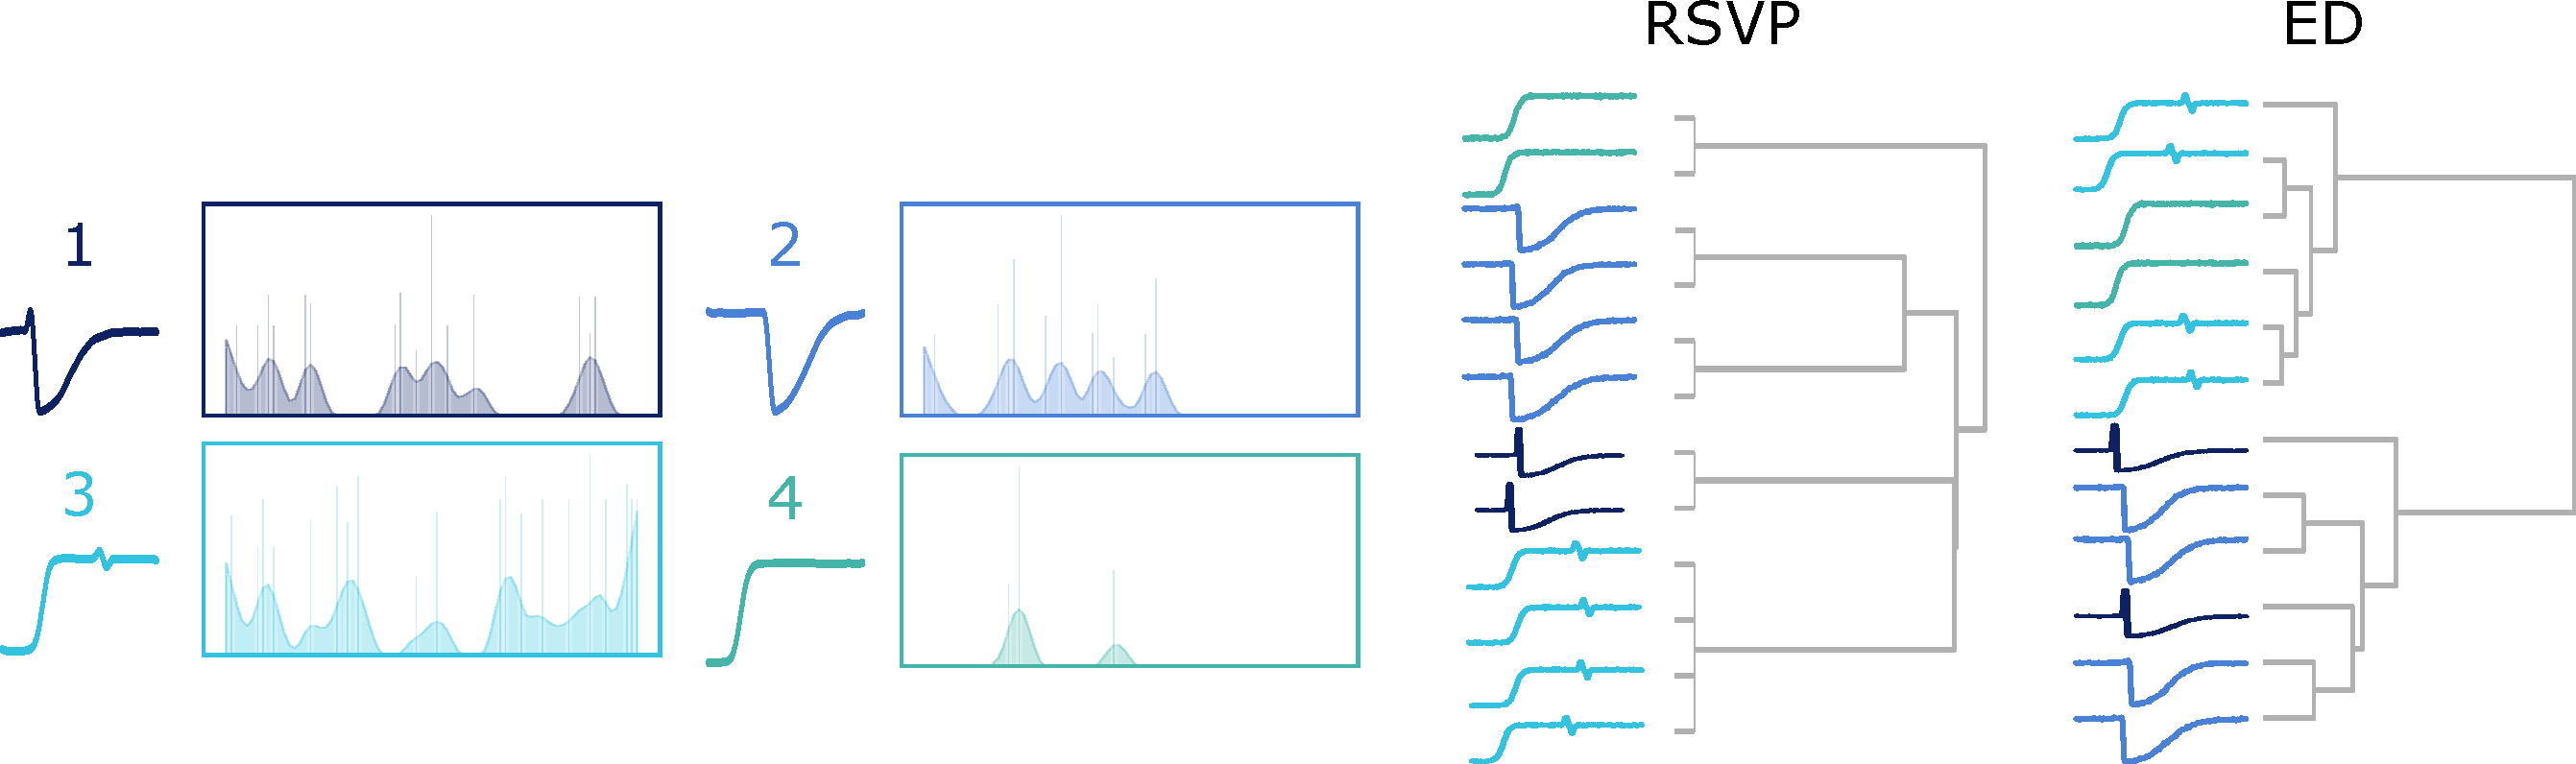
\includegraphics[width=\linewidth]{distribution_dendogram_ED_RSVP.pdf}
    \caption{}
    \label{fig:distribution_dendogram}
\end{figure}
 
As the reader can notice, the \gls{ED} mismatched signals from class 1 with signals from class 2, and signals from class 4 with signals from class 3. The fact that a misalignment between the main structures of the signals occur (the main peaks from signals of class 1 are misaligned and the main small peak and valley shapes of class 3 are slightly misaligned), increases the distance between signals that apparently have the same shape. In the other end, the proposed strategy follows a distance measure based on the presence(absence) of specific shapes, as well as how these are ordered (if \textit{n-grams} are used). This means that classes 1 and 2 will not be mismatched, because signals from class 1 have a peak whereas the ones from class 2 don't.

\subsection{Towards Interpretable Results}

Having demonstrated that it is possible to create a distance measure between time series with pure text, we highlight an advantage of working on the text domain, which is interpretability of the data. This advantage is taken because of the weighting factor attributed to each \textit{word} or \textit{n-gram} from the \gls{TFIDF} model. As explained by Pavel Senin \textit{et. al}, the weights can be used as a weighting vector for each word extracted, highlight the corresponding shape on the original signal and measuring its importance for the classification process \cite{sax_vsm}.

\begin{figure}
    \centering
    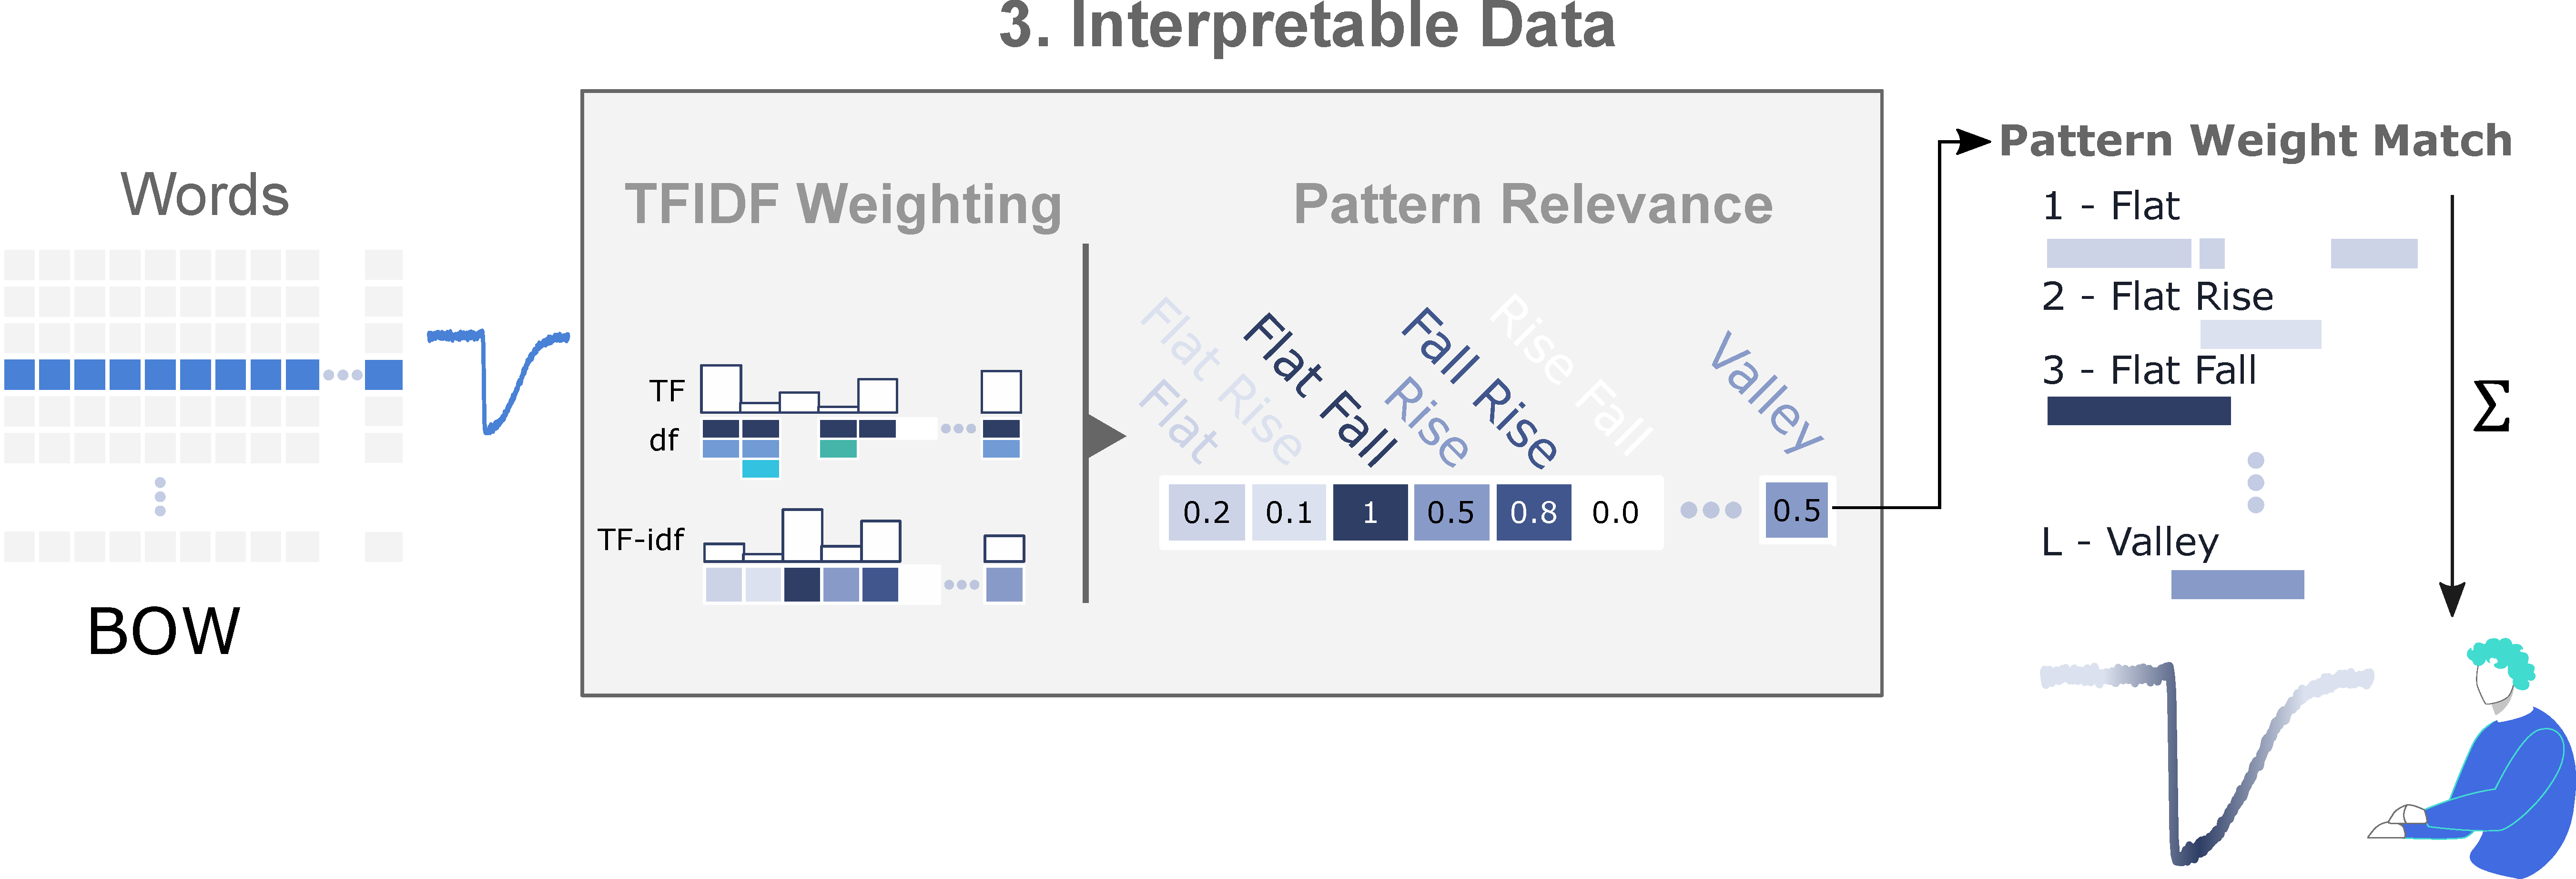
\includegraphics[width=\linewidth]{interpretable_scheme_explain.pdf}
    \caption{}
    \label{fig:distribution_dendogram}
\end{figure}

(IN THE FIGURE, SHOW THE PROCESS BY SEARCHING IN EACH TIME SERIES)

With this strategy we build a distribution of \textit{word} occurrences, which can be represented as an histogram that is a patch of a signal. The shape of histograms, shows very well how different two classes can be. This difference in distribution, as well as in relevance (with \gls{TFIDF}) is an interpretable result based on the description of the data, from which we can say: \textit{"class A is different than class B, because..."}.


This representation highlights the differences between classes and, as explained by Pavel Senin \textit{et. al}, can be used as a weighting vector for each word extracted and its importance for the classification \cite{sax_vsm}. In Figure \ref{fig:interp_data}, we show an illustrative example of the conversion of a BoW into a \textit{TF-IDF} matrix, and how the cumulative sum of weights onto the corresponding matches on the signal, are able to provide a human readable output, in addition to the text representation of the signal. 
\par
\textit{\textbf{Show an image with the distribution of words between classes with BoW and TFIDF to show the difference. Show as well how the weights can be used to represent one class over the other...}} 



\section{Towards Natural Language for Pattern Search}

Automobiles are increasingly monitoring every aspect of the driver’s behavior. Such data can be used for many direct and explicit purposes, such as optimizing fuel consumption or enhancing safety systems. However, there are also many potential indirect and offline uses of this data. The data may be of interest to engineers optimizing driver’s comfort, study the behavior of automated vehicles, to insurance companies fine-tuning insurance rates, to accident investigators trying to understand the cause of an accident, etc. [8,10–12,14,19]. It is commonly understood that individuals with domain experience can often “read” such telemetry. For example, in academic and industrial labs it is common to hear engineers annotate such data “This y-axis bump is where he hit the pothole, and then the sharp decline here in the x-axis is where he begins to apply the brakes” [22]. However, this ability to interpret such data does not help in searching such data collections. Simply manually panning through the data does not scale beyond minutes of data, and we may wish to search massive data archives.

\subsection{Mapping Features to Words}

We define a word feature vector W as a mapping of feature F with a specific word. With feature, we intend to describe either a property, such as the mean or standard deviation, but also a distance measure to pre-defined examples. In linguistic terms, this word feature vector is an adjective of the subsequence. Every subsequence Ti,m from each time series T is characterized by the selected set of words,  being created a set of word feature vectors for each time series, further normalized between 0 and 1. The word feature vector has the size of T minus the subsequence length: n-m+1, and the feature value indicates how relevant is the word in the subsequence. Figure 3 shows an example of the word feature vectors for up (Fup)and down (Fdown).

\textbf{SHOW FIGURE}

To allow interactive search, the word feature vectors are pre-computed in an offline indexing stage. In addition to this, we also extract three dimensions of the same word feature vector with different window lengths, based on m: W1→ m; W2→ \frac{m}{2}; W3→\frac{m}{4}; with the intent of matching ordered sequences of words inside a subsequence with the grouped followed by operator, as will be explained further. It is important to note that the ratio of the window used for the dimension W2 and W3 might have to be fine-tuned for the domain, as there might not be a “one window ratio fits all”. However, empirically we observed that the exact value of this ratio is not critical to the success of search.

For each W is assigned a word w. We use English words to make the process more intuitive, such as noise, up and peak. We recognize that the intuitive meaning of such words can vary from user to user depending on their domain, their experience and on the current context. Either way, words can be mapped to features that are domain specific or word feature vectors can be given a domain specific vocable, providing a more appropriate mathematical thinking behind what is its meaning. In addition, we are aware that multiple words can be given the same meaning and for this reason, we associate several synonyms to each word. We also note that our proposed mechanism can benefit from the current advances in Natural Language Processing (NLP). For instance, synonyms could automatically be associated with the closest word listed in our vocabulary with word embeddings. We defer such considerations to future work.

We define an initial subset of features that are mapped to words. When defining one word feature vector it would often come with a negation pair.

Definition 5 (Negation Pair): A negation pair (!W) represents the exact opposite of a defined word feature vector (W) following the rule:

\begin{equation}
!W = 1-W
\end{equation}


This indicates that when one increases the other one has to decrease proportionally. Examples of such word feature vectors are symmetric and asymmetric, or complex and simple. 

Note that some words might be the opposite of each other, but do not follow this rule, or even seem to be the opposite of each other, but are not. For instance, up and down are opposite of each other, but do not follow Equation 1. While one exists, the other can not, but it does not mean that when one is small, the other has to be high, since the subsequence might just be flat. Another case is the word peak. Intuitively, we would think that valley is the opposite of peak, but the consideration of !peak = valley is false. 

In this work, we use the negation of a word feature vector for cases where there is no negation pair. This negation is realized using an operator.



As previously noted, a set of features is used to extract several properties of all subsequences of a time series and attribute a semantic meaning to each one of them by mapping it to a specific word. It is our assumption that a subsequence can be mapped to a set of words that an analyst would use to describe it. Depending on the domain or vocabulary of the analyst, the set of words might have to be different and adjusted. Eventually, the dictionary can be expanded to other types of features and words. In any case, we want to demonstrate that this current set of words and operators can solve many transportation query search problems.
The initial subset of features is listed and described below. We divide the list of features in groups: local, global, and special. 

●	Local Features
○	up (down): The slope estimation of a linear adjustment (y= ax + b) to the subsequence, being up (down) = a, if aup>0 (adown <0) or up (down) = 0, if aup<=0 (adown >=0).
○	complex (simple): A complexity-invariant distance measure of the subsequence (simple = 1 - complex) [2].
○	noise (smooth): The residual error when modeled by a moving average (smooth = 1 - noise). 
○	symmetric (asymmetric): The MASS distance to the subsequence’s horizontally flipped self. 
○	peak (valley): The logarithmic MASS distance to the template of a peak (valley), modulated by a gaussian function.
○	stepup (stepdown): The logarithmic MASS distance to the template of a step-up(down) function;
○	plateauup (plateaudown): The logarithmic MASS distance to the template of a plateau-up(down) function;
○	uvalley (vvalley): The logarithmic MASS distance to the template of a U-shaped (V-shaped) valley function.

●	Global Features
○	top (bottom): The moving average of the time series (bottom = 1 - top);
○	high (low): The difference between the maximum and minimum value of a subsequence (low = 1 - high);
○	middle: The inverse of the distance to the average of the signal for each subsequence;
○	uncommon (common): The matrix profile of the time series (common = 1 - uncommon).

●	Special Feature
○	shape: The MASS distance profile of the time series with a query given by the user as an example. A word must be given as well, so that the shape can be integrated into the query language.    

Most of the word feature vectors are illustrated in Figure 4, with subsequences (in gray) from transportation telemetry data. 



\subsection{Linguistic Operators}

Definition 6 (Operator): The same way we use word and sentence connectors in our language to create contrast or attribute a temporal sequence, in our proposed system we use operators. An operator is a metacharacter or a word that can be used to diversify the way word feature vectors are handled, either in the way the information is extracted or how these are combined.  It contributes to a more versatile and expressive usage of this language. Currently, we have a simple list of four operators: negation (!), wild card (*), followed by, and grouped followed by (e.g., [W1 W2 … Ww This list can obviously be expanded and customized, but we want to demonstrate that with a minimal set of operators, most of the problems we present are solvable. 

Web search engines have many operators at the user’s disposal, but since a list of words is usually powerful enough to retrieve and correctly sort most of the desired results, very few (or none!) are often used. We believe that this is the case for this application as well but acknowledge that simple operators can make the query more natural and come in handy to perform conjunctions between features and multiple dimensions, such as temporal logic or negation. These operators are especially useful to close the gap between the query and human discourse, contributing to a more expressive mechanism when using the proposed language. Currently, four operators are available. Below is a list and description of each of them, starting with the negation operator (represented by the symbol  ! ).
•	Negation Operator  - !W : As mentioned above, most words come as an opposite pair, but some do not follow Equation 1. In these cases, or when the word has no direct opposite, it can be useful to penalize the presence of the word in a subsequence. This operator does that by applying Equation 1 to the word feature vector, W. 
When describing time series, we inevitably use temporal logic in explaining the sequence of shapes we perceive. 

The next operator is followed by.
 

Figure 4 – Examples of matches for most word feature vectors defined above, with subsequences from telemetry datasets. In gray are presented the subsequences that were used to generate the word feature vectors.
	A followed by B: This operator rewards a subsequence represented by A followed by one subsequence that has a high score for B, within a distance of size m. A and B can be single words, multiple words or even queries for different dimensions of the time series.

With this operator, we look ahead of a subsequence in the time series. However, in some cases, it might be useful to describe the sequence inside the limits of the window we defined. For these we have a special case of followed by, which is the grouped followed by ([ ]). 
	Grouped followed by ([W1 W2 … WN]): Instead of looking ahead in the time series, we look inside the subsequence to reward an ordered sequence of words. In this special case, the subsequence is segmented into N sub-windows, with size int(\frac{N}{m}), and the corresponding word is scored within this sub-window. For this, we use the other 2 dimensions of the word feature vectors (W2 and W3). If N<=3, W2 is used, while if N>3, W3 is used.
Often, within a subsequence, the differentiating property occurs on the first half, last third or another sub-window of the subsequence, while the remaining sub-window(s) is(are) not relevant. We therefore introduce the wildcard (*) operator.

•	Wildcard - * - The sub-window where * is used is valued equally for all subsequences.
As with vocabulary, the reader could imagine expanding our dictionary of operators, but even with a limited set of them, we are able to successfully solve all the proposed search tasks, which cover dozens of examples. 
After presenting the set of elements that can be used in QuoTS to query a pattern of interest, we are ready to explain how the query is turned into a score function and finally to a selection of the k-most relevant subsequences. 



\subsection{Natural Language Query for Time Series}


All words are stored in a vocabulary file, associated with a thesaurus file for synonym checks. When the user loads a signal to work on, all word feature vectors are extracted based on a specific window size and stored in memory. For each word, three sets of word feature vectors are stored (W1, W2 and W3) based on the original window size.  In case of having a MTS, all three sets of word feature vectors are extracted for each dimension. Having this set of information pre-computed helps make the search run at interactive speeds, even for large data collections. 
When all data is pre-computed, QuoTS is ready to accept queries by the user. The query field accepts any word available in the vocabulary and thesaurus. When any of the words are not present in our vocabulary, we alert the user which is the closest word available, based on edit distance. The query can accept operators and works for multidimensional querying. These are relevant elements that are used as a reference to parse the query into individual scoring elements. This parsing process is made by looking into: (1) which dimension(s) of the time series is (are) included; (2) which operators are used; and (3) the single written words. The first two define how the score is calculated, that is, how word feature vectors are combined, as well as which dimensions of the word feature vectors are used. For instance, when including multiple signals, the query parses which word(s) corresponds to which signal, to search for the correct index of word feature vectors in the pre-computed data. When the followed by operator is used, the query is parsed in which word(s) comes before and after it (this is applicable either if the operator is used for intra-signal or inter-signal search). Another element is the grouped followed by operator, which is parsed by identifying square brackets in the query.
When each of these elements are parsed, we end up with a single word or sequences of words, which are combined by summing their corresponding word feature vectors (this corresponds to an implicit OR). It is important to note that the score is calculated by adding together normalized scores for each parsed segment of the query. The reasoning is that each segment of the query should be weighted the same (e.g., if using the query noise [up down], as up and down are combined, the range of this segment is [0-2], while noise is [0-1]. Therefore, [up down] is normalized between [0-1] before being added to noise).  Finally, a score is given to each subsequence. The top k-subsequence are highlighted on the signal and sorted from highest to lowest. This process implies that trivial matches are not considered. As an example, if we want to search matches for the query s1: [up down] s2: flat, we parse it by signal, first computing the score function for s1 and s2 individually. Then, the score function of s1 will be normalized between [0-1] to then be added to the scoring function of s2.





